\documentclass[12pt,oneside]{uhthesis}
\usepackage{subfigure}
\usepackage[ruled,lined,linesnumbered,titlenumbered,algochapter,onelanguage]{algorithm2e}
\usepackage{amsmath}
\usepackage{amssymb}
\usepackage{amsbsy}
\usepackage{caption,booktabs}
\captionsetup{ justification = centering }
%\usepackage{mathpazo}
\usepackage{float}
\setlength{\marginparwidth}{2cm}
\usepackage{todonotes}
\usepackage{listings}
\usepackage{xcolor}
\usepackage{multicol}
\usepackage{graphicx}
\floatstyle{plaintop}
\restylefloat{table}
\addbibresource{Bibliography.bib}
% \setlength{\parskip}{\baselineskip}%
\renewcommand{\tablename}{Tabla}
\renewcommand{\listalgorithmcfname}{Índice de Algoritmos}
%\dontprintsemicolon
\SetAlgoNoEnd

\definecolor{codegreen}{rgb}{0,0.6,0}
\definecolor{codegray}{rgb}{0.5,0.5,0.5}
\definecolor{codepurple}{rgb}{0.58,0,0.82}
\definecolor{backcolour}{rgb}{0.95,0.95,0.92}

\lstdefinestyle{mystyle}{
    backgroundcolor=\color{backcolour},   
    commentstyle=\color{codegreen},
    keywordstyle=\color{purple},
    numberstyle=\tiny\color{codegray},
    stringstyle=\color{codepurple},
    basicstyle=\ttfamily\footnotesize,
    breakatwhitespace=false,         
    breaklines=true,                 
    captionpos=b,                    
    keepspaces=true,                 
    numbers=left,                    
    numbersep=5pt,                  
    showspaces=false,                
    showstringspaces=false,
    showtabs=false,                  
    tabsize=4
}

\lstset{style=mystyle}

\title{Extracción y estudio de la argumentación en la prensa cubana}
\author{\\\vspace{0.25cm}Luis Ernesto Ibarra Vázquez}
\advisor{\\\vspace{0.25cm}Damian Valdés Santiago}
\degree{Licenciado en Ciencia de la Computación}
\faculty{Facultad de Matemática y Computación}
\date{Fecha\\\vspace{0.25cm}\href{https://github.com/username/repo}{github.com/username/repo}}
\logo{Graphics/uhlogo}
\makenomenclature

\renewcommand{\vec}[1]{\boldsymbol{#1}}
\newcommand{\diff}[1]{\ensuremath{\mathrm{d}#1}}
\newcommand{\me}[1]{\mathrm{e}^{#1}}
\newcommand{\pf}{\mathfrak{p}}
\newcommand{\qf}{\mathfrak{q}}
%\newcommand{\kf}{\mathfrak{k}}
\newcommand{\kt}{\mathtt{k}}
\newcommand{\mf}{\mathfrak{m}}
\newcommand{\hf}{\mathfrak{h}}
\newcommand{\fac}{\mathrm{fac}}
\newcommand{\maxx}[1]{\max\left\{ #1 \right\} }
\newcommand{\minn}[1]{\min\left\{ #1 \right\} }
\newcommand{\lldpcf}{1.25}
\newcommand{\nnorm}[1]{\left\lvert #1 \right\rvert }
\renewcommand{\lstlistingname}{Ejemplo de código}
\renewcommand{\lstlistlistingname}{Ejemplos de código}

\begin{document}

\frontmatter
\maketitle

\begin{dedication}
A mis amigos y familia, a todas las personas que estuvieron en mi vida dando su apoyo y ayuda para superar los obstáculos.
\end{dedication}
\begin{acknowledgements}
    Agradecimientos
\end{acknowledgements}
\begin{opinion}
La lingüística computacional es una rama multidisciplinaria que procesa grandes 
cantidades de textos escritos. La tesis presentada por Luis Ernesto Ibarra Vázquez 
propone un algoritmo basado en modelos de aprendizaje automático para la segmentación 
y clasificación de enunciados argumentativos en textos de la sección “Cartas a la Dirección” 
del periódico \emph{Granma}.

La tesis se ubica en el marco de un proyecto \emph{Dinámicas sociales, políticas y económicas en el 
discurso público en Cuba de principio del siglo XXI: estudios de CORESPUC}, asociado al Programa 
Nacional de Ciencia y Técnica “Las Ciencias Sociales y las humanidades. Desafíos ante la estrategia 
de desarrollo de la sociedad cubana”, Código PN223LH011-011, Ministerio de Ciencia, Tecnología y 
Medio Ambiente (CITMA), Cuba, 2021-2023.

Por ello, Luis Ernesto tuvo que estudiar la materia referida, que no está incluida en el currículo 
de la carrera y trabajó mostrando creatividad, disciplina, entrega y rigor. Deseo destacar su 
profundización en el estudio computacional de la argumentación y la proposición de soluciones de 
software útiles para el análisis de enunciados argumentativos en español.

La investigación realizada por el estudiante incluyó diversos corpus en idioma inglés con 
diferentes anotaciones de la argumentación que se usaron para el entrenamiento de modelos de 
aprendizaje automático proyectivos para clasificar los enunciados argumentativos en español, a 
partir del conocimiento de la anotación en idioma inglés. Se compararon varios modelos y el mejor 
fue utilizado para la clasificación de enunciados de las Cartas a la Dirección del periódico Granma. 
Este trabajo es un primer paso positivo en el estudio automático de la argumentación de nuestra variante 
del español y llevará una posterior revisión por lingüistas. Dicho corpus anotado será importante para la 
realización de análisis sociolingüísticos del corpus donde la argumentación es una variable de interés para 
el proyecto CORESPUC.

Durante el desarrollo del trabajo, Luis Ernesto demostró habilidades para el trabajo con la bibliografía y 
creatividad para proponer soluciones a problemas de implementación, entre otras competencias de programación 
en el lenguaje Python y sus diversos \emph{frameworks}. Así, se logró cumplir el objetivo de esta tesis.

Por tanto, considero que al estudiante Luis Ernesto Ibarra Vázquez debe otorgársele la máxima calificación 
(5 puntos, Excelente), y estoy seguro que en el futuro Luis Ernesto se desempeñará como un excelente profesional 
de la Ciencia de la Computación.

\begin{flushright}

\includegraphics[scale=0.2]{Graphics/firma_enhanced.jpg}\\
MSc. Damian Valdés Santiago\\
21 de noviembre de 2022    
\end{flushright}

\end{opinion}
\begin{resumen}
% Resumen: IMRD, 250 palabras

% Introducción al problema
%  - Cuál es?
%  - Por qué es importante resolverlo?
% Cómo puede ser o es resuelto?
%  - Qué problemas tiene este proceso?
% Propuesta para mejorar el proceso de resolución del problema
%  - Modelo
%  - Resultados  

El estudio de la argumentación en la prensa cubana es un campo en donde se han reportado
relativamente pocas investigaciones. En estos estudios es posible obtener 
información de los esquemas argumentativos utilizados en los textos y
realizar acciones en base a estos.
Este problema tradicionalmente es resuelto mediante 
una anotación manual por expertos en lingüística, trabajo que se 
caracteriza por tomar mucho tiempo y recursos. La Extracción
de Argumentos es la rama del Procesamiento del Lenguaje Natural
encargada de estudiar algoritmos y métodos para solucionar los problemas
asociados a la anotación de las estructuras argumentativas. Mediante el uso 
de estos es posible automatizar el procedimiento de anotación
de la argumentación. 
En este trabajo se propone la anotación de textos argumentativos
mediante el uso de dos modelos de aprendizaje profundo, entrenados con 
conjuntos de datos traducidos y proyectados del inglés, encargados de resolver
las tareas relacionadas al problema. 
El primer modelo propuesto 
consiste en uno secuencia a secuencia usado para la extracción y clasificación
de las unidades de discurso argumentativas (UDA) mediante el uso de \emph{Long Short Term Memory} 
(LSTM) y \emph{Conditional Random Field} (CRF). Para la extracción y clasificación de 
enlaces entre las UDAs se propone un modelo de clasificación basado en redes residuales,
atención y LSTM. Ambos modelos utilizan \emph{embeddings} GloVe para la representación 
de las palabras. Los resultados obtenidos en la extracción de UDAs alcanzaron valores de
0,82 en la métrica F1 comparados con 0,85 obtenidos en el estado del arte. 
En las demás tareas, los resultados no son directamente comparables con los del estado del arte, 
los mejores valores F1 obtenidos fueron 0,56 en la clasificación de UDAs, 0,74 en la predicción
de enlaces y 0,39 en la clasificación de enlaces.
Con dichos modelos se anotaron las ``Cartas a la Dirección'', del 
periódico Granma, creándose un conjunto de datos con las estructuras argumentativas anotadas
y listas para el estudio de estas por lingüistas.

\end{resumen}

\begin{abstract}
	% Resumen en inglés

The study of argumentation in the Cuban press is a field in which relatively little
research has been reported. In these studies it is possible to obtain information on 
the argumentative schemes used in the texts and take actions based on them. This problem
is traditionally solved through manual annotation by linguistic experts, a work that takes 
a lot of time and resources. Argument Extraction is the branch of Natural Language Processing 
in charge of studying algorithms and methods to solve the problems associated with the annotation 
of argument structures. By using these algorithms it is possible to automate the argumentation 
annotation procedure.  In this paper we propose the annotation of argumentative texts by using 
two deep learning models, trained with translated and projected English datasets, in charge of 
solving the tasks related to the problem.  The first proposed model consists of a sequence to 
sequence one used for the extraction and classification of argumentative discourse units (ADUs) 
by using Long Short Term Memory (LSTM) and Conditional Random Field (CRF). A classification model 
based on residual networks, attention and LSTM is proposed for the extraction and classification of 
links between ADUs. Both models use GloVe for word representation. The results obtained in the 
extraction of ADUs reached values of 0.82 in the F1 metric compared to 0.85 obtained in the state 
of the art.  In the other tasks, the results are not directly comparable with those of the state of 
the art, the best F1 values obtained were 0.56 in UDAs classification, 0.74 in link prediction and 
0.39 in link classification. With these models, the ``Letters to the Management'' of the Granma 
newspaper were annotated, creating a data set with the argumentative structures annotated and 
ready to be studied by linguists. 

\end{abstract}
\tableofcontents
\listoffigures
% \listoftables
% \listofalgorithms
\lstlistoflistings

\mainmatter

\chapter*{Introducción}\label{chapter:introduction}
\addcontentsline{toc}{chapter}{Introducción}

La teoría de la argumentación o argumentación es el estudio interdisciplinario de cómo las conclusiones
pueden ser apoyadas o socavadas por premisas a través de razonamiento lógico (CITE Wikipedia English Argumentation Theory).
Esta es usada en varios aspectos de la vida como en las negociaciones, debates públicos, publicaciones
científicas, enseñanza, leyes. Todo argumento se compone escencialmente en un conjunto de premisas,
un método de razonamiento y una conclusión.


La Extracción de Argumentos es la rama del Procesamiento de Lenguaje Natural encargada de formularizar
y modelar dicho problema para su posterior procesamiento. Los modelos existentes generalmente se ecargan de
extraer y clasificar las componentes argumentativas y sus relaciones de una fuente no estructurada de 
texto, capturando un proceso de razonamiento y argumentación en su estructura final. Los métodos
de realizar este procedimiento varían en dependencia de las características en que se trabaja y el objetivo
a que se quiere llegar. Entre los métodos usados se pueden mencionar métodos ad-hoc basados en gramáticas,
que aprovechan atributos del texto como etiquetas POS y etiquetas de NER, que codifican diferentes 
patrones argumentativos (CITE Reconstructing Arguments from Noisy Text). Dicho enfoque requiere de trabajo 
humano para la creación de una gramática que permita resultados satisfactorios. Este tipo de enfoque
generalmente sacrifica recobrado por precisión y no permite una generalización del problema, contribuyendo
a no ser muy escalable. Otro método es el basado en técnicas de aprendizaje de máquina. Estos métodos están
divididos en diferentes vertientes de acuerdo a cómo procesan los datos. Uno de ellos lo realiza por
etapas, en el cual en cada una se resuelve independientemente los subproblema y la salida de la etapa 
anterior es entrada a la etapa siguiente. Las etapas en que generalmente se divide el problema
son, separación de unidades argumentativas y no argumentativas, clasificación de las unidades 
argumentativas y la identificación de estructuras argumentativas (CITE Identifying Argumentative Discourse Structures in Persuasive Essays, cualquier otro que use este enfoque).
Este enfoque trae consigo una modularidad elevada al resolver las tareas de manera independiente, pero
tiene la desventaja que los errores de etapas anteriores son pasados a las siguientes y además los algoritmos
usados no ven todo el contexto del texto pudiendo perder características que permitirían un mejor resultado.
Otro enfoque usado son los llamados end-to-end, en estos el modelo entrenado aprende los pasos para convertir
directamente la entrada del algoritmo en la salida deseada al entrenar sus diferentes partes de manera 
simultanea. En el contexto de EA la entrada serían los tokens de los textos y la salida sería las
estructuras argumentativas anotadas en dependencia del algoritmo usado. Este enfoque mitiga las posibles
deficiencias del enfoque por etapas, al juntar todo el proceso en una sola eliminando la propagación
del error, además de que al tener todos los datos es posible encontrar mayor cantidad de correlaciones 
entre ellos, también no requiere de una ingeniería de atributos (features) tan elaborada (CITE Neural End-to-End Learning for Computational Argumentation Mining).

En la práctica la EA tiene un gran número de aplicaciones: (CITE Argument Mining Linguistic Foundation pag 5)
\begin{itemize}
    \item Análisis de opinión: Ayuda no solo a saber si la opinión es favorable o no, sino a saber
    porqué es favorable o no.
    \item Análisis de debate: Ayuda a detectar estrategias argumentativas
    \item Detección de incoherencias en un conjunto de argumentos y justificaciones
\end{itemize}


En EA la gran mayoría de las investigaciones y corpus se basan en el idioma inglés o alemán. Hay
una cantidad pequeña de investigaciones en español (CITE Minería de argumentación en el Referéndum del 1 de Octubre de 2017) 
y basados específicamente en prensa no se encontró ninguna referencia. En Cuba no se tiene constancia
tampoco de investigaciones realizadas sobre el tema por lo que se considera la primera investigación
sobre las estructuras argumentativas en el país. El trabajo forma parte de una colaboración entre la 
Facultad de Artes y Letras de la Universidad de La Habana y la Facultad de Matemática y Computación 
de la misma universidad mediante el proyecto CORESPUC (TODO Poner el nombre completo del proyecto?).
Mediante este trabajo se podrá (TODO Poner acá para qué se quiere hacer el trabajo)


Este trabajo necesita encontrar \emph{qué modelos se pueden usar en el español para la extracción de 
argumentos en textos, especialmente en la prensa} (TODO Posible Pregunta Científica?). Recientemente se ha introducido modelos basados 
en Transformer y Attention (CITE Transformer-Based Argument Mining for Health Care Application, El doctorado)
que han llegado a alcanzar resultados iguales o superiores al estado del arte de su momento (TODO Posible Hipótesis?). 
Por otro lado dado que los corpus están en inglés se desea saber si \emph{es factible usar métodos
para poder usar el conocimiento aprendido de los algoritmos entrenados en inglés en el español} 
(TODO Posible Pregunta Científica).


El objetivo principal de este trabajo se basa sobre \emph{el diseño e implementación de un algoritmo para 
el estudio de la argumentación en el periódico digital Granma} (Objetivo). Para esto primero
es necesaria la construcción de un corpus sobre el periódico. Para esto se realizará una recolección
de noticias mediante técnicas de scrapping para conformar un corpus inicial no anotado. Este corpus
será anotado por un modelo previamente entrenado usando técnicas de proyección entre lenguajes (CITE Cross-lingual)
y otros tipos de anotaciones tales como partes de la oración y entidades presentes.

Actualmente existe un corpus parcialmente
anotado y con algunos errores documentados en la plataforma CQPweb (TODO Alguna referencia al corpus?,
Correcto poner CQPweb?) así que en una primera parte se realizará correcciones pertinentes a dicho 
corpus y luego se anotarán otros atributos relevantes como la clasificación de las secciones del 
periódico en de opinión o no. Luego se aumentará dicho corpus mediante técnicas de scrapping 
(TODO en español?) y se verificará la aparición o no de noticias entre la versión PDF y la versión 
online del periódico. Se necesita además la implementación de una interfaz visual en la cual se 
pueda consultar (TODO Consultar qué?) el corpus.


El trabajo está conformado por \dots (TODO Poner la estructura del trabajo)


% Esqueleto
% \begin{itemize}
%     \item Hablar sobre el conocimiento y el pensamiento del ser humano como ser racional.
%     No existe una verdad única, si no diferente tipos de verdades para diferentes grupos de personas.
%     Cada grupo de personas presentan argumentos por los cuales creen esas verdades y no creen otras.
%     \item Introducir el tema de la argumentación en el NLP, su usos actuales e importancia.
%     \item Introducción de la problemática (Formar un corpus de Granma con estructuras argumentativas),
%     el porqué se quiere hacer esto (Justificación del proyecto CORESPUC, crear un estudio en español del tema)
%     \item Hablar sobre la importancia teórica y práctica del trabajo. No existen estudios en español,
%     los corpus en español son escasos. Ayuda a resolver la justificación de CORESPUC
%     \item Planteo de los objetivos y las preguntas científicas (Crear corpus argumentativo en Español y un framework para la extracción de argumentos en periódicos)
%     \item Estructura del trabajo
% \end{itemize}


% Aspectos que debe tratar la introducción (Se deben de decir implícitamente en los párrafos):

% \begin{itemize}

%     \item Contexto histórico-social donde se desarrolla
%     \item Antecedentes del problema, justificación y motivación. Cómo se ha estudiado primero a mano y luego computacionalmente el problema en la prensa. Motivacion, el proyecto esta integrado en un proyecto nacional  reconocido CORESPUC, lo cual tiene una justificación también.
%     \item Breve presentación de la problemática. (No es el estado del arte aunque se puede hablar un poco de él) Elementos involucrados en el punto de vista cientifico, lleva corpus.
%     \item Actualidad, novedad e importancia teórica y práctica. Revisar literatura (Actualidad, en español no tiene mucho estudio), Se propone un modelo computacional para estudiar ese asutnto que se han propuesto poco, para Cuba no hay ninguno y poco de investigación. 
%     \item Diseño teórico.

%     \begin{itemize}

%         \item Problema: 
%         \item Objeto de Investigación: Procesamiento de Lenguaje Natural
%         \item Campo de acción: Linguistica computacional
%         \item Hipótesis o preguntas científicas
%         \item Objetivos generales y específicos

%         \begin{itemize}
%             \item General
%             \begin{itemize}
%                 \item Diseño e implementación de un algoritmo para el estudio de la argumentación en el periódico digital Granma
%             \end{itemize}
%             \item Específicos
%             \begin{itemize}
%                 \item Construcción del corpus de los periódicos: Crawler, Anotación (scpaCy).
%                 \item Arreglar etiquetas en corpus activo con archivos VRT.
%                 \item Clasificar las secciones en de opinión o no.
%                 \item Verificar la aparición o no de noticias entre la versión PDF y la versión online del periódico.
%                 \item Implementacion de la interfaz gráfica para consultar los resultados.
%                 \item Lograr interoperailidad de la plataforma CQPweb.
%             \end{itemize}
%         \end{itemize}

%     \end{itemize}

%     \item Estructura del trabajo

% \end{itemize}
\chapter{Argumentación}\label{chapter:argumentation}

% Argumentacion background

\section{Argumentación}

% TODO Ampliar esto, basarse en el articulo de MIT \cite{lawrence2020argument}

La argumentación es el proceso que consiste en producir elementos que justifiquen una afirmación. Una afirmación 
constituye una expresión de algo ocurrido, un juicio, una evaluación. Las premisas son los elementos que 
justifican o atacan las afirmaciones. Un argumento básico está dado por la relación entre una afirmación y una 
premisa, con dicha premisa estar atacando o apoyando la afirmación inicial. Un ejemplo básico constituye:

\begin{adjustwidth}{25pt}{25pt}
    \emph{Las vacunas previenen la diseminación de enfermedades}, por lo tanto \textbf{vacunarse es necesario}.
\end{adjustwidth}

En el ejemplo se puede observar un argumento simple y algunas características propias de estos, la justificación 
(en \textbf{negro}) que apoya la afirmación (en \emph{itálico}), también se puede observar palabras conectoras 
que indican además de conexión la dirección de esta.

Sobre esta han surgido diferentes marcos teóricos que buscan una metodología para su representación y estudio. 
Una de las más citadas constituye el Método o Modelo de Toulmin.

El Método Toulmin fue extrapolado del libro \emph{The Uses of Argument} [\cite{toulmin_2003}] escrito por Stephen E. Toulmin.
Este método divide los argumentos en seis partes: afirmación (claim), fundamento (grounds), 
justificación (warrant), calificador (qualifier), refutación (rebuttal) y respaldo (backing).
Mediante las afirmaciones se conoce el argumento principal que el autor quiere probar a la audiencia,
estas son respaldados con fundamentos siendo estos las evidencias y hechos en que se apoya el autor.
Las justificaciones pueden estar explícitas o implícitas y son suposiciones que vinculan los
fundamentos con las afirmaciones, estas a su vez pueden ser respaldadas por conocimiento.
El esquema introduce la posibilidad de otra sitaución válida a la establecida en las afirmaciones
mediante la refutación. Los calificadores son usados para dar más información de la calidad o seguridad
de las afirmaciones dadas. Un ejemplo de este esquema es:

\begin{adjustwidth}{25pt}{25pt}
    [\emph{Se escucharon ladridos y aullidos en la distancia}]$_{fundamento}$, 
    [\emph{probablemente}]$_{calificador}$ 
    [\emph{haya perros en las cercanías}]$_{afirmación}$.
\end{adjustwidth}

En este ejemplo, además de las partes explícitas, se encuentran implícitas como la justificación 
(los perros son animales que ladran y aullan), el respaldo (se sabe que existen perros en la zona) y 
la refutación (Puede ser que hayan lobos o coyotes cerca). [\cite{toulminArgument}]
  
\section{Extracción de Argumentos}

El Procesamiento de Lenguaje Natural (\textbf{NLP} por sus siglas en inlgés \emph{Natural Language Processing}) es un 
subcampo de la Inteligencia Artificial (IA) que tiene como objetivo la comprensión del lenguaje humano por 
las computadoras. 
Mediante el uso de sus algoritmos es posible el procesamiento masivo de texto para la extracción de información 
relvante de este. Entre las tareas pertenecientes a dicho campo se encuentran Traducción Automática, 
Generación de Lenguaje Natural y Extracción de Argumentos (EA). La EA constituye la identificación y extracción 
automática de las estructuras de inferencia y 
razonamiento expresadas como argumentos presentes en el lenguaje natural [\cite{lawrence2020argument}].
En la actualidad en tareas de \textbf{NLP} como análisis de sentimientos permiten 
extraer cuales son las opiniones o sentimientos presentes, este análisis, sin embargo, presenta una falta 
de información, ya que no presenta el porqué de estas. La EA permite dar respuesta a este problema presentando
los argumentos y cómo sus relaciones justifican sus posiciones.

\subsection{Estructuras Argumentativas}

% TODO HAblar de esquemas argumentativos? Esto seria las clasificaiones seleccionadas para las UDA y relaciones
% además del método para segmentación de UDA y el criterio de marcar las relaciones

Las estructuras argumentativas son las partes y sus relaciones de las cuales están compuestas la argumentación en los textos.
Estas se componen de dos elementos principales, las Unidades de Discurso Argumentativas (UDA) y los enlaces
existentes entre estas. Las UDAs presentan varias definiciones en las que se ven como cláusulas, oraciones, aunque
todas estas se presentan como secciones consecutivas de texto que no se sobreponen. Estas UDAs se relacionan entre 
sí formando el proceso de inferencia y razonamiento.
Tanto los enlaces como las UDAs son clasificadas en dependencia de su rol en la argumentación, estas clasificaciones 
parten de los conceptos de premisa y afirmación para las UDA y ataque y apoyo para las relaciones. 

\subsection{Tareas de extracción de argumentos}

Dada las estructuras argumentativas en la EA se conciben las siguientes tareas principales:

\subsubsection{Extracción de UDAs}

Esta tarea constituye en la separación de los segmentos de texto que formarán parte de la estructura.
El texto entrado es segmentado y como salida se obtiene un conjunto de UDAs. En el siguiente ejemplo se 
pone un ejemplo de la extracción de UDAs (en \emph{itálico}).

\begin{adjustwidth}{25pt}{25pt}
    Existen muchos efectos de la expansión de la tecnología en la transportación y las comunicaciones,
    las cuales son mencionanadas ahora. En primer lugar, [\emph{el correo electronico puede contar como uno de los resultados
    más beneficiosos de la tecnología moderna}]. [\emph{Años atrás, las personas pagaban gran cantidad de dinero para 
    enviar sus cartas y sus pagos estaban sujetos al peso de sus cartas o paquetes y muchos accidentes podrían 
    causar problemas que causarían que el correo no fuera enviado}].
\end{adjustwidth}

\subsubsection{Clasificación de UDAs}

La clasificación de UDAs consiste en asignarle el papel que toma la UDA en la argumentación. En general 
las clasificaciones parten de dos clases bases, las afirmaciones, las cuales son posiciones que toma el 
autor del texto y las premisas, que son datos, eventos, elementos que se consideran verdades por sí solas.  

\begin{adjustwidth}{25pt}{25pt}
    Existen muchos efectos de la expansión de la tecnología en la transportación y las comunicaciones, 
    las cuales son mencionanadas ahora. En primer lugar, [\emph{el correo electronico puede contar como uno de los resultados
    más beneficiosos de la tecnología moderna}]$_{Afirmación}$. [\emph{Años atrás, las personas pagaban gran cantidad de dinero para 
    enviar sus cartas y sus pagos estaban sujetos al peso de sus cartas o paquetes y muchos accidentes podrían 
    causar problemas que causarían que el correo no fuera enviado}]$_{Premisa}$.
\end{adjustwidth}

\subsubsection{Extracción de relaciones entre las UDAs}

La extracción de relaciones constituye en determinar si estan relacionadas las UDAs. La disposición de estas
relaciones forma el proceso de razonamiento en que se basa el autor para validar su posición. En el ejemplo 
se representa la existencia de relación mediante su distancia argumentativa con la UDA con la que se relaciona.
La distancia argumentativa son la cantidad de UDAs del texto que separan la UDA fuente del objetivo [\cite{galassi2018argumentative}], 
en caso de ser negativa el objetivo se encuentra antes que la fuente y viceversa.

\begin{adjustwidth}{25pt}{25pt}
    Existen muchos efectos de la expansión de la tecnología en la transportación y las comunicaciones, 
    las cuales son mencionanadas ahora. En primer lugar, [\emph{el correo electronico puede contar como uno de los resultados
    más beneficiosos de la tecnología moderna}]$_{Afirmación}$. [\emph{Años atrás, las personas pagaban gran cantidad de dinero para 
    enviar sus cartas y sus pagos estaban sujetos al peso de sus cartas o paquetes y muchos accidentes podrían 
    causar problemas que causarían que el correo no fuera enviado}]$_{Premisa, -1}$.
\end{adjustwidth}

\subsubsection{Clasificación de relaciones entre las UDAs}

Los tipos de relaciones, nacen de dos clases bases por lo general, están las relaciones de apoyo y las de ataque.
Las de apoyo se centran en aquellas en las que la UDA fuente afirme la UDA objetivo, las de ataque se basan en 
las que la UDA fuente apoye la negación de la UDA objetivo.

\begin{adjustwidth}{25pt}{25pt}
    Existen muchos efectos de la expansión de la tecnología en la transportación y las comunicaciones, 
    las cuales son mencionanadas ahora. En primer lugar, [\emph{el correo electronico puede contar como uno de los resultados
    más beneficiosos de la tecnología moderna}]$_{Afirmación}$. [\emph{Años atrás, las personas pagaban gran cantidad de dinero para 
    enviar sus cartas y sus pagos estaban sujetos al peso de sus cartas o paquetes y muchos accidentes podrían 
    causar problemas que causarían que el correo no fuera enviado}]$_{Premisa, -1, apoyo}$.
\end{adjustwidth}

Partiendo de esto, se puede observar que las estructuras argumentativas de un texto constituyen un grafo dirigido 
en donde sus nodos representan las UDA y están anotados con su tipo y sus vértices representan las 
relaciones entre las UDA y dichos vértices se anotan con el tipo de relación existente entra ambas (\ref{fig:arg_struct}).

\begin{figure}[h!]
	\begin{center}
		\begin{center}
			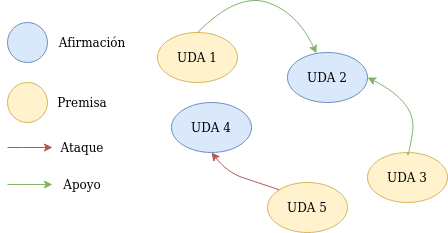
\includegraphics[scale=.7]{Graphics/Estructuras_argumentativas.png}
            % \includesvg[options]{Graphics/Estructuras argumentativas.svg}
        \end{center}
	    \caption{Estructuras Argumentativas}
	\end{center}
\end{figure}\label{fig:arg_struct}

\chapter{Propuesta}\label{chapter:proposal}

El modelo propuesto se divide en dos secciones. En la primera sección se realiza la segmentación y clasificación de 
las UDAs como tareas conjuntas. En la segunda sección se predicen los enlaces y sus clasificaciones, tomando
como tareas auxiliares la clasificación de las UDAs. Dada la heterogeniedad de las conjuntos de datos disponibles 
en EA, los modelos poseen un mínimo de atributos, esto permite que el modelo por sí solo aprenda 
la mejor representación para el esquema de anotación con que se entrene.

\section{Segmentación y clasificación de UDAs}

Esta primera parte se modela como un problema secuencia a secuencia cuyo objetivo es asignar a los tokens 
extraídos del documento entrada una etiqueta BIOES para segmentar las UDAs. Para la clasificación del tipo 
de UDA, al conjunto de etiquetas BIES se le añadieron las clasificaciones que presenta el corpus entrenante.
En el siguiente ejemplo se muestra una salida del modelo presentando las clasificaciones de
$A$ como argumento y $P$ como premisa:

\begin{adjustwidth}{25pt}{25pt}
    En$_O$ primer$_O$ lugar$_O$ ,$_O$ [\emph{el$_{B-A}$ correo$_{I-A}$ electrónico$_{I-A}$ puede$_{I-A}$ 
    contar$_{I-A}$ como$_{I-A}$ uno$_{I-A}$ de$_{I-A}$ los$_{I-A}$ resultados$_{I-A}$
    más$_{I-A}$ beneficiosos$_{I-A}$ de$_{I-A}$ la$_{I-A}$ tecnología$_{I-A}$ moderna$_{E-A}$}] .$_{O}$ 
    [\emph{Años$_{B-P}$ atrás$_{I-P}$ ,$_{I-P}$ las$_{I-P}$ personas$_{I-P}$ pagaban$_{I-P}$ gran$_{I-P}$ cantidad$_{I-P}$ 
    de$_{I-P}$ dinero$_{I-P}$ para$_{I-P}$ enviar$_{I-P}$ sus$_{I-P}$ cartas$_{I-P}$ y$_{I-P}$ sus$_{I-P}$ 
    pagos$_{I-P}$ estaban$_{I-P}$ sujetos$_{I-P}$ al$_{I-P}$ peso$_{I-P}$ de$_{I-P}$ sus$_{I-P}$ 
    cartas$_{I-P}$ o$_{I-P}$ paquetes$_{I-P}$ y$_{I-P}$ muchos$_{I-P}$ accidentes$_{I-P}$ podrían$_{I-P}$
    causar$_{I-P}$ problemas$_{I-P}$ que$_{I-P}$ causarían$_{I-P}$ que$_{I-P}$ el$_{I-P}$ correo$_{I-P}$ 
    no$_{I-P}$ fuera$_{I-P}$ enviado$_{E-P}$}] .$_{O}$
\end{adjustwidth}

\subsection{Modelo de segmentación y clasificación de UDAs}

Sea $D$ un documento entrada, este es separado en una secuencia de $n$ tokens $D_i$ donde $n$ es la mayor longitud encontrada
en los documentos del conjunto de datos (si la cantidad de tokens es menor que $n$ entonces $D_i$ es completado con un token especial de enmascarado). 
A cada token se le asigna
su representación vectorial GloVe de dimensión $g=300$, dando como resultado $G_{ij} \in \mathbb{R}^{n \times g}$.
Esta representación inicial presenta información semántica de las palabras y conserva las relaciones 
espaciales entre ellas. 

Para la representación de información morfológica de la palabra se construyen dos
codificadores que procesan los caracteres de cada token y devuelven una representación vectorial de estos.
A cada caracter se le asigna un vector que será entrenado convirtiendo un token en un vector de dimensión
$q \times c$, donde $q$ es el tamaño máximo de palabra en el conjunto de datos y $c$ es la dimensión del vector
asignado a cada caracter.
Uno de estos modelos está basado en CNN, este modelo entrena una representación de caracteres de dimensión
$cd=50$ representando un token como un vector de dimensión $q \times cd$. Se conforma por una capa de convolución unidimensional
con $f=30$ filtros y un kernel de tamaño $k=3$, seguida por una capa \emph{max pooling} que convierte la secuencia en un vector
de dimensión $1 \times f$, que luego es concatenado a la representación del token a que pertenece.
Otro modelo utilizado para calcular una representación morfológica se encuentra basado en RNN. Se usó
un modelo LSTM bidireccional con dimensión $l=25$ para calcular la representación del token, para las dimensiones de los caracteres se
utilizan vectores de tamaño $l$, el resultado final constituye la concatenación de la corrida hacia adelante y
hacia atrás formando una representación de dimensión $1 \times 2 \cdot l$ del token. Este vector es concatenado a la representación
del token correspondiente. Otro atributo usado en la representación de los tokens constituyen las etiquetas de 
Partes de la Oración de estos.
El conjunto de etiquetas elegido es un conjunto universal [\cite{petrov2011universal}] aplicable a cualquier idioma.
De estas etiquetas se les extrae la codificación \emph{one-hot} y esta es transformada por una capa densa con $p=5$ neuronas
y función de activación \emph{ReLU}, el resultado es concatenado a la representación del token correspondiente. Mediante 
la extracción de estos atributos el token es representado en tres maneras, semántica, morfológica y estructural, con el 
objetivo de que sean aprendidas los rasgos lingüísticos correspondientes a la tarea.

Del proceso de vectorización sale un vector con dimensión $n \times t$ donde $t$ es la dimensión final de la representación
de los tokens. Este vector es modificado por una capa LSTM bidireccional de dimensión $m=200$, a esta salida se le 
añade una conexión residual al ajustarle la dimensión con una capa densa. Luego, la secuencia es procesada por una 
capa densa de dimensión $k=100$ con activación \emph{ReLU} produciendo una representación final de dimensión 
$n \times k$. Finalmente, se utiliza una capa CRF
para la clasificación final de la secuencia en las etiquetas finales. El resultado final constituye un vector
de dimensión $n$ que representa las clasificaciones inferidas por el modelo (Figura \ref{fig:segmenter_model}).

Para prevenir el sobreajuste se agregaron capas de normalización y de \emph{dropout} entre cada proceso y se usaron regularizaciones
L2 y \emph{dropout} en las capas densas y LSTM, el valor asignado al dropout es de $0.5$. 
Para prevenir el sobreentrenamiento se aplicó una 
terminación temprana de este cuando no se encontraba una mejora de la función de pérdida en el conjunto de validación
por más de 10 épocas consecutivas. Como optimizador se utilizó Adam con una tasa de aprendizaje de $0.001$.

\subsection{Posprocesamiento de segmentación y clasificación de UDAs}

La salida del modelo constituye una secuencia de etiquetas en formato BIOES. Esta está propensa
a contener errores en su formato, por ejemplo, secuencias no terminandas en E, segmentos continuos con más de una 
meta-etiqueta, entre otros.
Para la corrección de la estructura se propone el siguiente algoritmo con dos partes. La primera
consiste en arreglar la estructura BIOES, para esto se mantiene una ventana de tamaño
3, [\_ , \_ , \_], sobre la secuencia y se asume que la parte anterior a la posición de la ventana no presenta errores. Al encontrar una
ventana inválida se necesita observar la siguiente ventana para poder decidir cómo se arregla el error, ya que se
podría dar el caso que se observe [O, O, I] y la próxima sea [O, I, O], en donde solamente viendo la primera ventana no se podría saber si el cambio 
correcto corresponde a sustituir I por B o por S. Una vez observadas las dos ventanas, se procede a realizar el 
arreglo correspondiente. En casos donde sea ambigua la manera de arreglar la ventana, [I, I, O] por ejemplo
(La I o la O pueden ser 
sustituidas por una E), se utiliza una función que recibe un segmento y devuelve la gravedad del error.
El error con mayor gravedad será arreglado, en caso de ser iguales se arreglará la etiqueta más a la izquierda.
Este procedimiento devuelve una secuencia BIOES correctamente anotada, debido a que a partir de una secuencia sin 
errores en cada paso se va arreglando la ventana y una vez esta llega al final arregló todos los elementos de la secuencia.
Una vez la secuencia tiene la estructura BIOES correctamente anotada el problema
consiste en arreglar las meta-etiquetas, ya que una misma secuencia BIOES pudo haber sido anotada con diferentes
tipos, en este caso se toma la etiqueta más representativa del segmento continuo.

\begin{figure}[p]
	\begin{center}
		\begin{center}
            \includesvg[scale=.65]{Graphics/Modelo_Segmenter_UDA.svg}
        \end{center}
	    \caption{Segmentador UDAs.}\label{fig:segmenter_model}
	\end{center}
\end{figure}

\newpage

\section{Predicción y clasificación de enlaces}

En esta segunda parte el modelo se encarga de las tareas de extracción y clasificación de enlaces.
El problema consiste en clasificar pares de UDAs, representando origen y objetivo del enlace, 
en el tipo de relación que existen entre estas.
Como tarea auxiliar se clasifican los tipos de UDAs que intervienen en la relación. La salida 
del modelo constiuye en una tupla de tres elementos: la clasificación de la relación, 
la clasificación de la UDA origen, la clasificación de la UDA objetivo. Si el enlace existe o no 
es calculado partir de la clasificación de la relación.   

\subsection{Modelo de predicción y clasificación de enlaces}

Sean dos UDAs, $S$ y $T$, donde $S$ representa la fuente de la relación, mientras que $T$ representa
al objetivo. Estas secuencias son tokenizadas y se les asigna la representación GloVe de cada palabra, obteniendo
dos vectores de dimensión $u \times g$, donde $u$ es el tamaño máximo de UDAs en el conjunto de entrenamiento
y $g=300$ es la dimensión del \emph{embedding}.
Estos vectores son modificados por una red densa compuesta por $ca = 4$ capas con activación \emph{ReLu}
de dimensiones $50$, $50$, $50$, $300$, añadiendo una conexión residual a la salida de esta. 
El próximo paso consiste en aplicar una capa densa de dimensión $di=50$ y luego un \emph{average pooling}
de tamaño $dp=10$, obteniendo vectores de dimensión $\frac{q}{dp} \times di$. 
Estos vectores son modificados por un LSTM bidireccional con $lm=50$ unidades. Un módulo de atención es aplicado 
sobre los vectores fuentes, 
en este actúan como consultas el promedio de los vectores objetivo y como llaves y valores los vectores fuentes,
el procedimiento simétrico es realizado para los vectores objetivos.
La salida de los procesamientos son concatenados con la distancia argumentativa obteniendo una representación 
conjunta de la relación a analizar. Esta representación conjunta es modificada por una red residual obteniendo
una representación final de dimensión $l=20$ y luego sometida a los clasificadores de relación y de tipos de UDAs
(Figuras \ref{fig:link_predictor_model1} y \ref{fig:link_predictor_model2}).

Para prevenir el sobreajuste se agregaron capas de normalización y de \emph{dropout} entre cada 
proceso y se usaron regularizaciones L2 y \emph{dropout} en las capas densas y LSTM, 
todos los \emph{dropout} tienen valor $dr=0,1$. Para prevenir el sobreentrenamiento se aplicó una 
terminación temprana de este cuando no se encontraba una mejora de la función de pérdida en el 
conjunto de validación durante $v=5$ épocas consecutivas. Como optimizador se utilizó Adam con descenso 
exponencial con tasa de aprendizaje $lr=0.003$.

Dado que se realiza un aprendizaje de varias tareas, se tienen varias funciones de pérdida individuales que conforman 
la función de pérdida final $e$. Sea $e_r$ la función de pérdida de la clasificación de la relación, $e_s$ la del tipo de UDA origen  
y $e_t$ del tipo de UDA objetivo, entonces $e = 10 \cdot e_r + e_s + e_t$.

\subsection{Preprocesamiento de predicción y clasificación de enlaces}

El uso de este modelo se concreta a nivel de documento, en donde ya se tienen las UDAs extraídas. Para alimentar
al modelo con los pares de UDAs y sus distancias argumentativas se seleccionan todos los pares de estos que cumplan
que no se enlacen con ellos mismos, por ejemplo, $a \rightarrow a$; y que su distancia argumentativa absoluta sea menor 
que $da=10$. Estas restricciones disminuyen el número de pares extraídos por documentos a una cantidad lineal 
con respecto a la cantidad de UDAs, presentes ya que por cada UDA solamente se tomarían $2 \cdot da$ elementos como máximo
(los que la preceden y los que la suceden). 

Además de las etiquetas $R$ originales del conjunto de entrenamiento, se añaden elementos extras a este
conjunto. Estos elementos son las representaciones inversas de las relaciones, por ejemplo, si $a \xrightarrow{c} b$ entonces 
se agregará el par $b \xrightarrow{c^{-1}} a$, donde $c^{-1}$ es una nueva clasificación de relación que representa
el inverso de la clasificación $c$. Este proceso se realiza para aumentar la cantidad de relaciones positivas en el
conjunto entrenante, ya que aun con las reducciones hechas existe un desbalance de clases positivas y negativas en
las relaciones.

\subsection{Posprocesamiento de predicción y clasificación de enlaces}

Se calcula una salida extra a partir de las distribuciones de probabilidad de las relaciones 
devueltas por el modelo, esta salida representa si el par está enlazado o no directamente, para este cálculo se 
suman las categorías vinculadas a las clases originales del conjunto de datos, esta se toma como la probabilidad de estar 
enlazados, que en caso de ser mayor del 50\% se devuelve verdadero. Para dar el resultado final se eliminan del 
conjunto de respuesta las relaciones anotadas con las etiquetas inversas añadidas en el paso de preprocesamiento 
y son devueltas aquellas que se clasifiquen como enlazadas según el criterio anterior.

\newpage

\begin{figure}[p]
    \begin{center}
        \includesvg[scale=.6]{Graphics/Modelo_Link_Prediction1.svg}
        \caption{Predictor de enlaces.}\label{fig:link_predictor_model1}
    \end{center}
\end{figure}
\begin{figure}[p]
    \begin{center}
        \includesvg[scale=.6]{Graphics/Modelo_Link_Prediction2.svg}
    \end{center}
    \caption{Predictor de enlaces (continuación).}\label{fig:link_predictor_model2}
\end{figure}

\chapter{Experimentación}\label{chapter:implementation}

En el capítulo se describen los conjuntos de datos utilizados para el entrenamiento y validación del modelo 
propuesto y cómo se construyen los conjuntos de datos en español. Se mencionan las herramientas utilizadas 
para la confección del software. Además, se describe el 
proceso de experimentación y evaluación de los modelos construídos con los conjuntos de datos. Finalmente,
se presentan los resultados obtenidos al aplicarles los modelos a las Cartas a la Dirección extraídas 
del periódico Granma. 

\section{Conjuntos de Datos}

Para el entrenamiento de los modelos propuestos se utilizaron corpus diferentes, estos
presentan esquemas de anotación distintos entre sí, difieriendo principalmente en la definición de UDA y 
las clasificaciones dadas a estas y a las relaciones. A todos los conjuntos se les proyectó al lenguaje 
español y se les realizó un aumento de datos. Como conjunto para la validación fueron usadas 
una parte de las Cartas a la Dirección del periódico Granma.

\subsection{Ensayos Argumentativos}\label{corpus:persuasive_essays}

Este corpus [\cite{stab2017parsing}] presenta unos 402 documentos, dividido por los autores en 286 documentos para entrenamiento (70\%), 
80 para prueba (20\%) y 36 para validación (10\%). Los contenidos de estos son ensayos de estudiantes en los que 
se argumentan sobre temas como cooperar o competir y contribuciones de la tecnología a la sociedad.
Las anotaciones de las UDAs se conforman por segmentos de textos argumentativos, estos segmentos son 
clasificados en \emph{MajorClaim} (751, 12\%), \emph{Claim} (1506, 25\%) y \emph{Premise} (3832, 63\%).
La estructura de las relaciones entre las UDAs conforman árboles en los que se tienen como raíz las 
\emph{MajorClaim} del texto. Las relaciones solo están permitidas entre \emph{Premise-Premise} y \emph{Premise-Claim}, clasificadas
en \emph{attack} (219, 6\%) y \emph{support} (3613, 94\%). Las relaciones entre \emph{Claim} y \emph{MajorClaim} son anotadas 
de manera diferente, por medio de 
darle a las \emph{Claim} una clasificación de si está a favor (1228) o en contra (278) de las \emph{MajorClaim} del documento.
Para el análisis de este corpus se consideraron las relaciones \emph{Claim-MajorClaim} de igual manera que las otras,
al convertir estas posiciones en relaciones. El número final con la inclusión de estas aumenta a 715 (10\%) de ataque y 
5958 (90\%) de apoyo.

\subsection{CDCP}\label{corpus:cdcp}

El corpus [\cite{niculae2017argument}] está conformado por 731 comentarios de usuarios extraídos de la web bajo el tema de 
prácticas de cobro de deudas a los consumidores (CDCP en inglés).
Las UDAs se encuentran segmentadas en oraciones y todas se consideran argumentativas, estas son clasificadas en 
\emph{policy} (815, 17\%), \emph{value} (2180, 45\%), \emph{fact} (785, 16\%), \emph{testimony} (1116, 21\%) y \emph{reference} (32 1\%). 
Las relaciones se encuentran clasificadas en \emph{reason} (1352, 97\%) y \emph{evidence} (73, 3\%).

\subsection{AbsTRCT}

AbsTRCT [\cite{mayer2020transformer}] se compone de 500 documentos sobre el estudio de cuatro enfermedades diferentes,
glaucoma, hipertensión, hepatitis b y diabetes. Las UDAs constituyen oraciones, aunque no todas son consideradas
argumentativas. Estas se clasifican en \emph{MajorClaim} (93, 3\%), \emph{Claim} (993, 30\%) y \emph{Premise} (2198, 67\%).
Las relaciones están representadas por tres categorías: \emph{support} (1763, 85\%), \emph{partial-attack} (238, 12\%) y
\emph{attack} (60, 3\%).

En resumen, estos datos no son grandes y contiene una gran cantidad de desbalance en sus clases.
En la Tabla \ref{table:corpus_info} se muestran los datos promedio de la composición de los diferentes corpus. 
Se observa una composición heterogenea entre estos, principalmente CDCP difiere en gran número de los demás.

\begin{table}[h!]
	\begin{center}
		\scalebox{0.8}{
		\begin{tabular}{|c|c|c|c|c|} \hline
		Corpus		            & Tokens 	& Tokens argumentativos	& UDAs   & Relaciones por UDA    \\ \hline
		Ensayos Argumentativos  & 381		& 68\% 					& 35\% 	 & 1,08					 \\ \hline
		CDCP		            & 127		& 99\% 					& 97\% 	 & 0,30					 \\ \hline
		AbsTRCT	                & 371		& 50\% 					& 47\% 	 & 0,63					 \\ \hline
		\end{tabular}
		}
	\caption{Información de promedios de los conjuntos de datos.}\label{table:corpus_info}
	\end{center}
\end{table}

\subsection{Creación de corpus en español}

\subsubsection{Aumento de datos}

% TODO PREGUNTAR Dice poner {back-translation} aunque en la referencia original lo dice junto
A los conjuntos de datos a analizar se les realizó un aumento de datos mediante le técnica de \emph{backtranslation},
aplicándole la proyección de etiquetas de los elementos originales a los aumentados.
Esto contribuyó a duplicar la cantidad de elementos disponibles. Los resultados obtenidos al comparar los 
elementos originales con los aumentados se reflejan en la Tabla \ref{table:data_augmentation}.
Estos muestran que se logró una variación pequeña en los datos, aunque conservando la 
longitud original del texto. 

\begin{table}[h!]
	\begin{center}
		\scalebox{1}{
		\begin{tabular}{|c|c|c|c|c|} \hline
		Corpus		            &  Jaccard	& Levenshtein	& $\frac{|\mathrm{Palabras} \quad \mathrm{originales}|}{|\mathrm{Palabras \quad aumentadas}|}$   \\ \hline
        Ensayos Argumentativos	&  0.69		                & 96		                    & 1.00	  \\ \hline
		CDCP                    &  0.72	                    & 30		                    & 1.02	  \\ \hline
        AbsTRCT                 &  0.74		                & 86		                    & 1.04	  \\ \hline
		\end{tabular}
		}
	\caption{Datos promedios comparando los textos originales con los aumentados.}\label{table:data_augmentation}
	\end{center}
\end{table}

\subsubsection{Proyección de corpus}

Todos los conjuntos de datos están originalmente en inglés, por lo tanto, se les aplicó el algoritmo de proyección
de corpus para obtener uno en español para ser usado en el entrenamiento de los modelos. 
Para la traducción automática se utilizó el servicio de Google Translate\footnote{\href{https://translate.google.com/}{https://translate.google.com/}}. 
Para calcular las 
alineaciones de palabras se probaron dos algoritmos: FastAlign [\cite{dyer2013fastalign}] y AwesomeAlign 
[\cite{dou2021word}]. Se observó que el primero, aunque es más rápido posee una calidad menor en los resultados,
el segundo posee una mayor calidad, aunque requiere de mayor tiempo y recursos para ejecutarse. Para los experimentos
se usó finalmente AwesomeAlign. La proyección de las etiquetas fue llevada a cabo por el algoritmo propuesto 
% TODO Cite problem, citar como texto
% [\autocite{eger2018cross}] 
% [\parencite{eger2018cross}] 
% [\citet{eger2018cross}] 
% [\citep{eger2018cross}] 
en \textcite{eger2018cross}.

\subsection{Cartas a la Dirección}

Las Cartas a la Dirección constituyen un segmento del periódico Granma donde son publicadas
cartas enviadas por la población o empresas a dicha entidad. En general, las cartas 
presentan dudas o problemas de la población con el objetivo de obtener respuestas del organismo
asociado. Se extrajeron 2891 cartas desde el 30 de agosto del 2013 hasta el 28 de octubre del 2022. Estas 
contienen aproximadamente 975000 palabras en los datos, en promedio, la cantidad de palabras por carta es de 330.
Se encontraron 874 cartas en respuesta a cartas enviadas, lo que representa un 30\% del total. Se extrajeron
los comentarios asociados a las cartas, en este sentido 987 cartas no presentan comentarios y, en promedio, 
se realizan 2 comentarios por carta. Los textos presentan un título y un formato relativamente libre, 
aunque en las cartas de respuesta se puede observar una firma de la persona que respondió y la entidad que 
representa. Del total de cartas, se seleccionaron las que fueran en respuesta a otra y también las 
cartas que fueron respondidas para tener una mayor concentración de cartas que fueran argumentativas, 
esta selección está conformada por 1702 cartas, lo que representa un 59\% del total de cartas.

\section{Implementación}

La implementación de los modelos y algoritmos de procesamiento y visualización de datos se encuentran en 
un repositorio de GitHub\footnote{\url{https://github.com/luisoibarra/argument-mining}}. Esta implementación
está concebida para que se pueda extender fácilmente para el uso con otros idiomas diferentes del inglés y el 
español. Se basa en una arquitectura de procesamiento secuencial en el cual cada paso del proceso realiza
una tarea específica y lo más desacoplada posible de las otras. Las tareas realizadas son:

\begin{itemize}
    \item Creación del corpus en un formato estándar: dado que los corpus vienen en diferentes 
	formas, este paso se realiza para trabajar sobre una misma representación de este.
    \item Proyección del corpus de un lenguaje fuente a un lenguaje objetivo: en el caso de 
	uso del trabajo se proyecta del inglés al español.
    \begin{itemize}
        \item Traducción y alineación de oraciones.
        \item Alineación de palabras.
        \item Proyección de etiquetas.
    \end{itemize}
    \item Extracción y clasificación de UDAs.
    \item Extracción y clasificación de las relaciones entre las UDAs.
    \item Visualización de los resultados.
\end{itemize}

\subsection{Herramientas}

El lenguaje empleado para la confección del software fue Python [\cite{python}], este presenta 
una gran variedad de herramientas 
para el trabajo con texto, visualización de datos y creación de modelos de aprendizaje profundo.
Se utilizó tensorflow [\cite{tensorflow}] en su versión 2.9.2 para la construcción y entrenamiento de los modelos. 
Para el procesamiento de los textos se utilizaron nltk [\cite{nltk}] y spacy [\cite{spacy}], con estos se realizaron tareas
como la extracción de tokens y oraciones del texto, la anotación de las etiquetas de partes de la oracion. Se utilizaron 
ambos paquetes para el procesamiento debido a que, en dependencia de la situación, cada uno presenta diferentes
ventajas. En el caso de nltk, presenta algoritmos rápidos para el procesamiento de texto que no 
requieren de muchos recursos computacionales, sin embargo, estos algoritmos no están disponibles de inmediato
para otros lenguajes como el español. Spacy por su parte presenta algoritmos más certeros a costo 
de mayor tiempo de procesamiento y gasto de recursos computacionales, y también presenta una cantidad mayor de lenguajes 
disponibles. Para la visualización y manejo de los datos, y cálculo de métricas se utilizaron 
matplotlib [\cite{matplotlib}], pandas [\cite{pandas}] y sklearn [\cite{sklearn}]. 
Para la recolección de las Cartas a la Dirección del periódico Granma se utilizó scrapy [\cite{scrapy}].
Como interfaz visual para el usuario se utilizó la herramienta Brat [\cite{brat}] 
(Figura \ref{fig:brat_persuasive_granma_letters}). Esta herramienta permite
la visualización y edición de las estructuras argumentativas. Dado que Brat es una página web, esta se puede
desplegar y permite su uso online.

\begin{figure}[h!]
	\begin{center}
		% 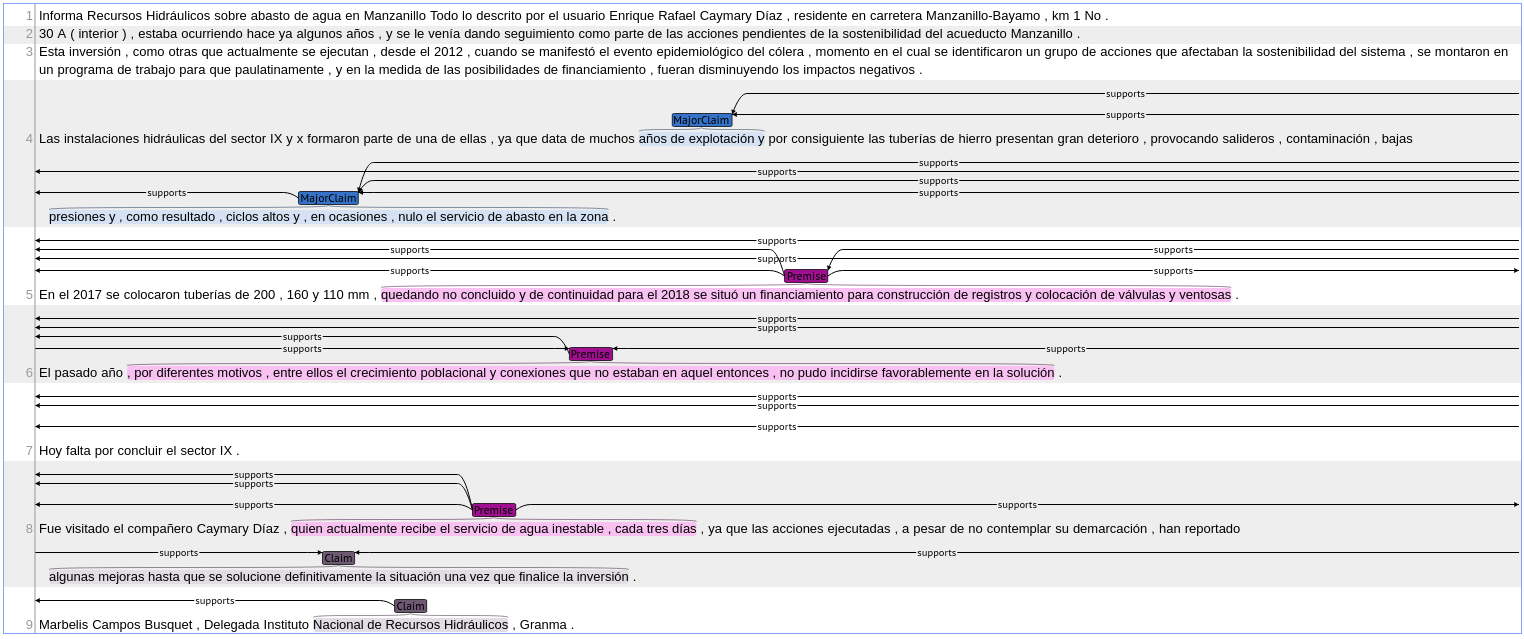
\includegraphics[scale=.4]{Graphics/persuasive_2019-01-25|informa-recursos-hidraulicos-sobre-abasto-de-agua-en-manzanillo|abasto-de-agua-en-manzanillo.png}
		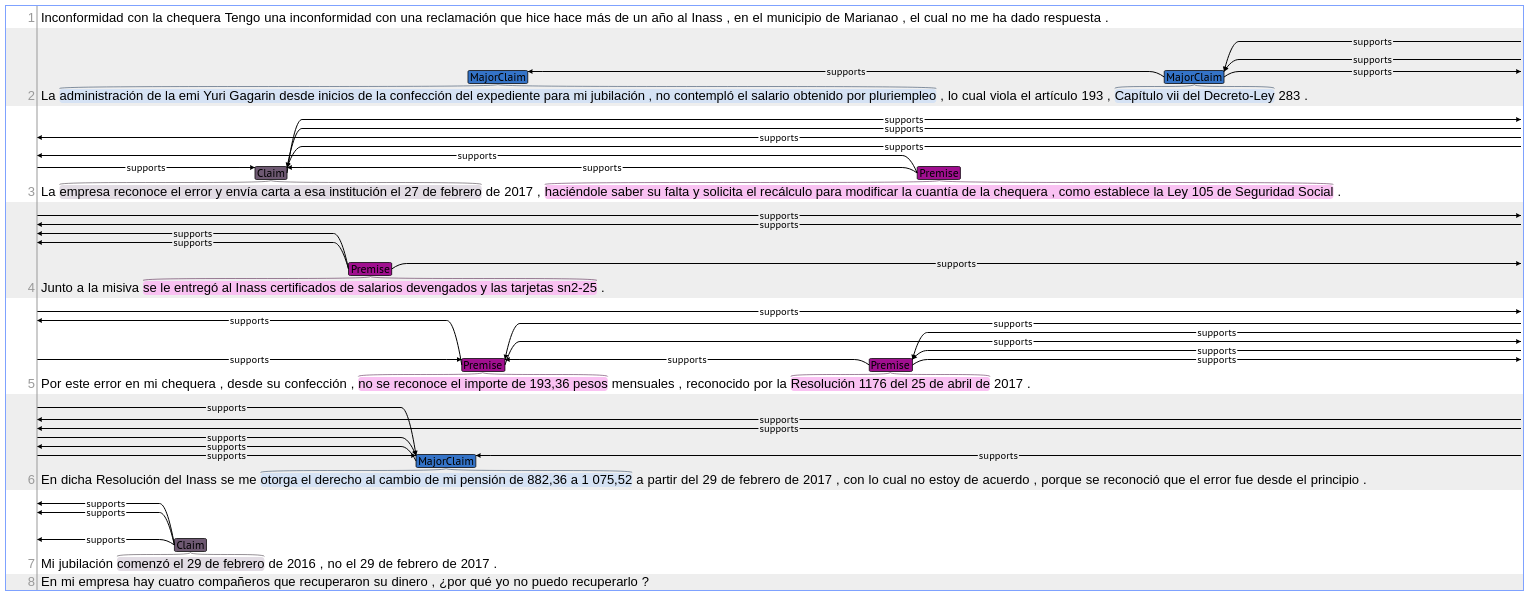
\includegraphics[scale=.4, width=435pt, height=250pt]{Graphics/persuasive_2019-03-22|inconformidad-con-la-chequera.png}
		\caption{Visualización con Brat de las estructuras argumentativas.}\label{fig:brat_persuasive_granma_letters}
	\end{center}
\end{figure}

\subsection{Formato Estándar}

El formato estándar creado es basado en el esquema de anotación CoNLL, donde se anotan a nivel de token todos los aspectos 
relavantes para las tareas a realizar. La segmentación de las UDAs son representadas por las anotaciones 
BIO o BIOES en cada palabra, en adición, las clasificaciones de estas son anotadas al adicionar el nombre 
de esta separada por un guión. Las relaciones son anotadas auxiliándose de la distancia argumentativa, estas 
son agregadas al anotar el tipo de relación con su respectiva distancia ambas separadas por un guión. A 
continuación se muestran ejemplos de este formato, conformado por el token, su clasificación BIOES, su clasificación
UDA, y las relaciones representadas por su clasificación y su distancia argumentativa:

\begin{itemize}
	\item Elemento fuera de una UDA: $análisis \quad O$
	\item UDA intermedia con una relación: $contribuye \quad I-Premise-attacks-5$
	\item Inicio de UDA con dos relaciones: $atletas \quad B-Claim-attacks--1-attacks-12$
\end{itemize}

\section{Experimentación}

Para realizar la selección del modelo se utilizó el corpus de Ensayos Argumentativos. Con este se ajustaron
las arquitecturas e hiperparámetros de los modelos propuestos. La mejor combinación de estos fue utilizada 
para el entrenamiento de los corpus restantes. Finalmente, los modelos fueron utilizados para anotar las Cartas 
a la Dirección. 

\subsection{Hardware}

Gran parte del procesamiento se llevo a cabo en una computadora $i5$ con $8GB$ de RAM ampliada con $4GB$ de memoria 
\emph{swap} [\cite{swap}], aunque se requirió el uso de la plataforma Colab [\cite{colab}] para 
el entrenamiento de algunos modelos por falta de recursos locales.

\subsection{Segmentador de UDA}

En el entrenamiento del segmentador de UDA se hicieron variaciones en la arquitectura propuesta con respecto a la
presencia o no de las siguientes componentes, presentando cuatro candidatos (Tabla \ref{table:segmenter_architecture_table}):

\begin{itemize}
    \item Atributos de POS en la entrada del algoritmo (POS).
    \item Atributos extraídos por la CNN de la palabra (Char-CNN).
    \item Atributos extraídos por la LSTM bidireccional de la palabra (Char-LSTM).
    \item Conexiones residuales (Res).
    \item Capa densa final (Densa).
    \item Capas de normalizaciones (Norm).
\end{itemize}

\begin{table}[h!]
	\begin{center}
		\begin{tabular}{|c|c|c|c|c|c|c|} \hline
		Modelos 		& POS       & Char-CNN  & Char-LSTM & Res       & Norm      & Densa  \\ \hline
		Modelo 1		& $\times$	& $\times$    & $\times$    & $\times$	& $\times$    & $\times$ \\ \hline
		Modelo 2		& $\times$	& $\checkmark$    & $\checkmark$    & $\checkmark$	& $\checkmark$    & $\times$ \\ \hline
		Modelo 3		& $\checkmark$	& $\checkmark$    & $\checkmark$    & $\checkmark$	& $\checkmark$    & $\times$ \\ \hline
		Modelo 4		& $\checkmark$	& $\checkmark$    & $\checkmark$    & $\checkmark$	& $\checkmark$    & $\checkmark$ \\ \hline
		\end{tabular}
	\caption{Variantes de arquitectura de los modelos de segmentación de UDA.}\label{table:segmenter_architecture_table}
	\end{center}
\end{table}

En la Figura \ref{fig:segmenter_model_loss} se observan las diferentes curvas de aprendizaje de los modelos 
probados. Se muestra la rápida convergencia de los modelos con conexiones residuales y normalizaciones.
Se muestra también la tendencia al sobreajuste en el entrenamiento entre los pasos 17-20, en donde se detiene el 
entrenamiento para evitar el crecimiento del error de generalización.

\begin{figure}[h!]
	\begin{center}
		\begin{center}
			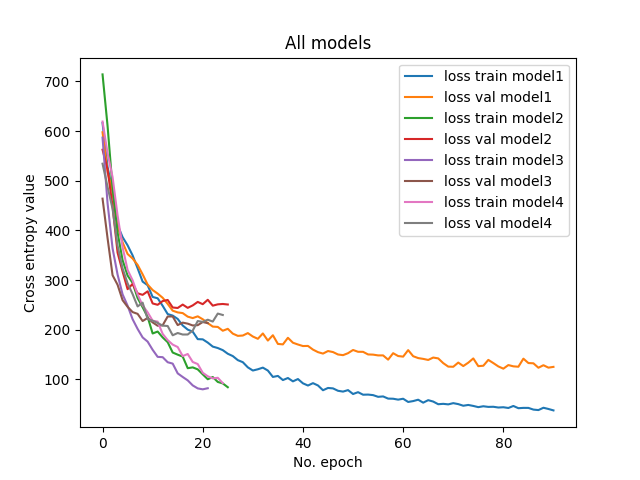
\includegraphics[scale=.7]{Graphics/persuasive_essays_all_linked_crf_loss.png}
        \end{center}
	    \caption{Pérdida de los modelos segmentadores.}\label{fig:segmenter_model_loss}
	\end{center}
\end{figure}

Las métricas 100\%F1 y 50\%F1 muestran que los modelos 1 y 2 presentan un desempeño menor que los 3 y 4. 
Se muestra un ligero aumento de 1\% en las 50\%F1 en el modelo 4 con respecto 
al modelo 3, aunque las métricas de F1 en el 3 superan a las de 4. Se considera a la 
segmentación como tarea principal, por lo que se selecciona como mejor modelo al 4 (Figura \ref{fig:test_segmenter_model_metrics}).
Las distinciones BIOES en los nombres de tablas o métricas constituyen la métricas correspondientes 
a la segmentación estrictamente, mientras las que no poseen dicha distinción sontituye al proceso 
conjunto de segmentación y clasificación de UDAs. 

\begin{figure}[h!]
	\begin{center}
		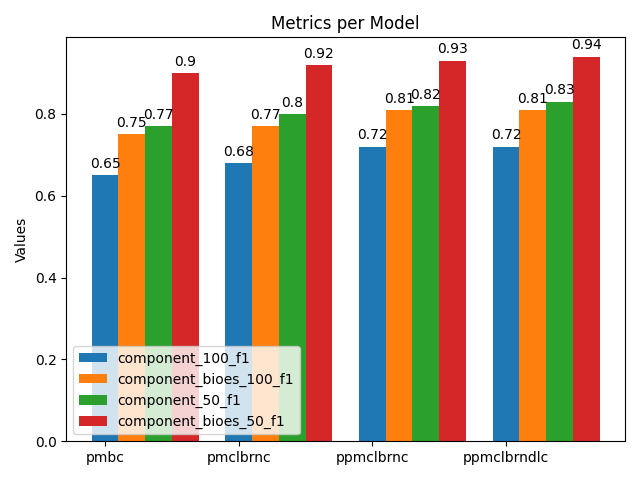
\includegraphics[scale=.4]{Graphics/persuasive_essays_all_linked_components.png}
		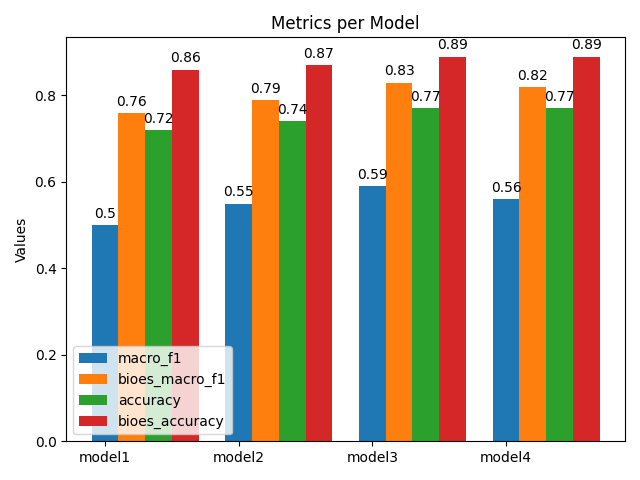
\includegraphics[scale=.4]{Graphics/persuasive_essays_all_linked_macro_micro_metrics.png}
	    \caption{Métricas del conjunto de pruebas de los modelos segmentadores.}\label{fig:test_segmenter_model_metrics}
	\end{center}
\end{figure}

El modelo seleccionado fue usado en el entrenamiento de los demás conjuntos de datos obteniendo los resultados mostrados
en Tabla \ref{table:test_metrics_segmenter} y Tabla \ref{table:test_bioes_metrics_segmenter}.

\begin{table}[h!]
	\begin{center}
		\scalebox{0.9}{
		\begin{tabular}{|c|c|c|c|c|c|} \hline
        Corpus		            & F1 Ponderado  & Macro F1	& \emph{Accuracy} & 100\%F1 & 50\%F1  	   \\ \hline
        Ensayos Argumentativos  & 0,76          & 0,56 		& 0,77		      & 0,72    & 0,83       \\ \hline
        CDCP		            & 0,65          & 0,45 		& 0,66		      & 0,61    & 0,68       \\ \hline
        AbsTRCT	                & 0,86          & 0,50 		& 0,87		      & 0,61    & 0,75       \\ \hline
        \end{tabular}
		}
	\caption{Métricas de las pruebas del segmentador de UDA.}\label{table:test_metrics_segmenter}
	\end{center}
\end{table}
\begin{table}[h!]
	\begin{center}
		\scalebox{0.9}{
		\begin{tabular}{|c|c|c|c|c|c|} \hline
        Corpus		            & F1 Ponderado  & Macro F1 & \emph{Accuracy} & 100\%F1 &  50\%F1   \\ \hline
        Ensayos Argumentativos  & 0,89          & 0,82	   & 0,89            & 0,81	   & 0,94 	   \\ \hline
        CDCP		            & 0,95          & 0,56	   & 0,96	         & 0,82	   & 0,93 	   \\ \hline
        AbsTRCT	                & 0,90          & 0,79	   & 0,91	         & 0,66	   & 0,82 	   \\ \hline
        \end{tabular}
		}
	\caption{Métricas BIOES de las pruebas del segmentador de UDA.}\label{table:test_bioes_metrics_segmenter}
	\end{center}
\end{table}

\subsection{Predictor de Enlaces}

Para el modelo se realizó un voto conjunto del ensamblado de 3 modelos, dado que el entrenamiento 
está basado en la aleatoriedad, se entrenan los modelos con los mismos datos obteniendo inferencias no
necesariamente iguales.
Para la selección del modelo se entrenaron diferentes variantes de arquitecturas e hiperparámetros, y 
al igual que en el segmentador de UDAs se realizó la selección del modelo que mejor se desempeñó en 
el conjunto de datos de Ensayos Argumentativos. De las variaciones surgieron las siguientes propuestas
(Tabla \ref{table:link_predictor_architecture_table}):

\begin{table}[h!]
	\begin{center}
		\scalebox{0.85}{
		\begin{tabular}{|c|c|c|c|c|c|c|} \hline
		Modelos   	 & Atención      & Pooling  & \emph{Dropout}   & Tasa de aprendizaje & Paciencia & Devolver mejores     \\ \hline
		Modelo 1	 & $\times$	     &  5       & 0,5               & 0,0015               & 10	      & $\checkmark$        \\ \hline
		Modelo 2	 & $\times$	 	 & 10       & 0,1               & 0,003                & 5	      & $\times$            \\ \hline
		Modelo 3	 & $\checkmark$	 &  1       & 0,1               & 0,003                & 5	      & $\times$            \\ \hline
		Modelo 4	 & $\checkmark$	 &  1       & 0,5               & 0,0015               & 10	      & $\checkmark$        \\ \hline
		\end{tabular}
		}
	\caption{Variantes de arquitectura de los modelos de predicción de enlaces.}\label{table:link_predictor_architecture_table}
	\end{center}
\end{table}

Las curvas de aprendizaje del proceso de entrenamiento de los modelos (Figura \ref{fig:link_prediction_model_loss}) 
muestran un nivel de sobreajuste 
elevado que disminuyen cuando el \emph{dropout} aumenta. Además, se observan valores de pérdida elevados lo que significa 
que al modelo le cuesta ajustarse de manera satisfactoria a los datos.

\begin{figure}[h!]
	\begin{center}
		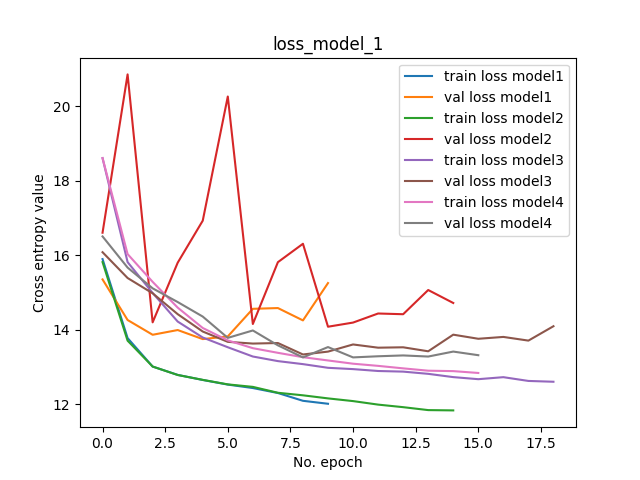
\includegraphics[scale=.7]{Graphics/persuassive_essays_all_linked_link_prediction_loss_model_1.png}
	    \caption{Curvas de aprendizaje de los modelos de predicción de enlaces.}\label{fig:link_prediction_model_loss}
	\end{center}
\end{figure}

Las métricas obtenidas por las diferentes versiones de los modelos 
(Figura \ref{fig:link_prediction_model_metrics}) 
muestran que el modelo 2 constituye una opción ligeramente superior en lo correspondiente a 
predicción de enlace a los otros modelos. Esos hiperparámetros
fueron utilizados para el entrenamiento con los demás conjuntos de datos.

\begin{figure}[h!]
	\begin{center}
		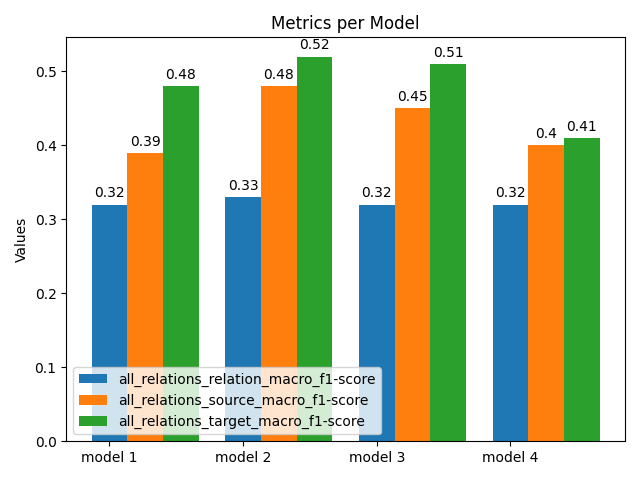
\includegraphics[scale=.4]{Graphics/persuasive_essays_all_linked_all_relation_f1_scores.png}
		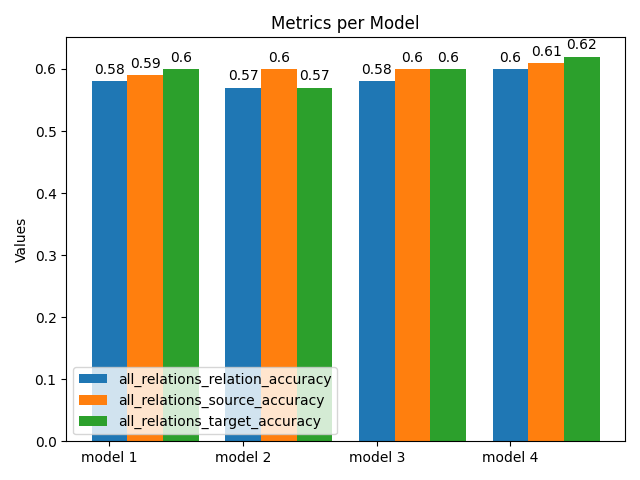
\includegraphics[scale=.4]{Graphics/persuasive_essays_all_linked_all_relation_accuracy.png}\\
		\text{a)$\qquad \qquad \qquad \qquad \qquad \qquad \qquad \qquad $b)}
	\end{center}
	\begin{center}
		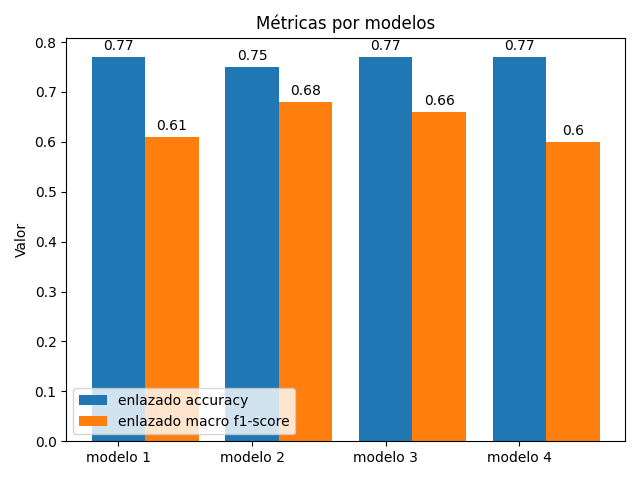
\includegraphics[scale=.4]{Graphics/persuasive_essays_all_linked_all_relation_linked.png}\\
		\text{c)}
	\end{center}
	\caption{Métricas F1 de la clasificación de enlace (a), \emph{accuracy} (b) y
			F1 de la predicción de enlace (c) de los modelos de predicción de enlaces.}
	\label{fig:link_prediction_model_metrics}
\end{figure}

En el entrenamiento del modelo en los demás conjuntos de datos se obtuvieron los resultados de las Tablas 
\ref{table:test_relation_metrics_link_predictor} y \ref{table:test_source_metrics_link_predictor}.

\begin{table}[h!]
	\begin{center}
		\scalebox{0.9}{
		\begin{tabular}{|c|c|c|c|c|} \hline
        Corpus		            & Macro F1 & \emph{Accuracy} & Macro F1 Enlace  & \emph{Accuracy} Enlace  \\ \hline
        Ensayos Argumentativos  & 0,33	   & 0,57            & 0,68	    		& 0,75	    		  	  \\ \hline
        CDCP		            & 0,37	   & 0,63	         & 0,79	    		& 0,68	    		  	  \\ \hline
        AbsTRCT	                & 0,39	   & 0,61	         & 0,83	    		& 0,74	    		  	  \\ \hline
        \end{tabular}
		}
	\caption{Métricas de predicción de relaciones de las pruebas del predictor de enlace.}\label{table:test_relation_metrics_link_predictor}
	\end{center}
\end{table}

\begin{table}[h!]
	\begin{center}
		\begin{tabular}{|c|c|c|c|} \hline
        Corpus		            & F1 Macro  & \emph{Accuracy} \\ \hline
        Ensayos Argumentativos  & 0,48       & 0,60             \\ \hline
        CDCP		            & 0,26       & 0,52	         \\ \hline
        AbsTRCT	                & 0,51       & 0,79	         \\ \hline
        \end{tabular}
	\caption{Métricas de predicción de fuente de las pruebas del predictor de enlace.}\label{table:test_source_metrics_link_predictor}
	\end{center}
\end{table}

\begin{table}[h!]
	\begin{center}
		\begin{tabular}{|c|c|c|c|} \hline
        Corpus		            & Macro F1 & \emph{Accuracy} \\ \hline
        Ensayos Argumentativos  & 0,52	   & 0,57             \\ \hline
        CDCP		            & 0,36	   & 0,54	         \\ \hline
        AbsTRCT	                & 0,53	   & 0,81	         \\ \hline
        \end{tabular}
	\caption{Métricas de predicción de objetivo de las pruebas del predictor de enlace.}\label{table:test_target_metrics_link_predictor}
	\end{center}
\end{table}

\subsection{Acoplamiento de los modelos}

Dado que la clasificación de UDAs es hecha tanto en el segmentador como en el predictor de enlaces, es necesaria 
la selección de cómo se va a desambiguar esta clasificación. En caso de seleccionar el predictor de enlaces como 
clasificador final, surgen varias cuestiones, como por ejemplo, que las UDAs pueden tomar varias clasificaciones o el
predictor no toma el contexto del texto completo en la clasificación. Aunque la primera puede ser corregida
mediante la selección de la clase más votada o algún otro criterio, la segunda presenta un mayor problema. Por
esto es seleccionada la clasificación del segmentador como etiqueta final para las UDAs y el predictor es usado para 
la tarea de extracción y clasificación de relaciones.

\subsection{Comparación con el estado del arte}

Las comparaciones se realizan por conjuntos de datos y se muestran las 
métricas indicadas por los autores de cada propuesta. Cada corpus y propuesta 
presenta características únicas que hacen que comparaciones directas sean 
difíciles de realizar, por lo tanto, la información brindada muestra una comparación 
cualitativa y no cuantitativa en la mayoría de los casos. 

Una de las principales dificultades está dada por el hecho de que las métricas calculadas son de la versión proyectada
al español, lo cual contribuye a variaciones en las etiquetas finales debido al lenguaje mismo 
o a errores en el proceso. Otros ejemplos en la dificultad de comparar las métricas se encuentra
en los enfoques tomados por las investigaciones anteriores a la hora de realizar las tareas.
En algunos casos la segmentación se presenta como una tarea de clasificación BIO, o simplemente 
se separan por oraciones y las clasifican en argumentativas o no. En el aspecto de clasificación
de las UDAs se emplean métodos como su clasificación independiente luego de ser extraída o su modelación
conjunta con la segmentación. En la extracción y clasificación de relaciones se observan técnicas de 
optimización de problemas enteros, clasificación por SVM o también probando los posibles enlaces dos 
a dos independientemente.

En la comparación de métodos se seleccionaron seis métricas que evalúan las diferentes 
tareas de la EA. La métrica BIOES F1 se refiere 
a la Macro F1 de la clasificación de las etiquetas BIOES, esta constituye una medida
que califica la tarea de segmentación de UDAs en el texto. La métrica Clas UDA F1 es 
calculada como la Macro F1 de las etiquetas BIOES junto con las etiquetas del tipo de 
UDA, medida que evalúa la tarea de clasificación de las UDAs. Rel Pred F1 es la medida 
Macro F1 de la predicción de enlaces y Rel Clas F1 la de la clasificación, estas 
son calculadas tomando en cuenta todos los pares seleccionados para el conjunto de 
datos. En la comparación $\checkmark$ significa que son directamente comparables,
$*$ que el método de comparación es el mismo, pero no son usados los mismos 
elementos para calcular la métrica, y $\times$ que la métrica no se encontraba disponible.

\begin{table}[h!]
	\begin{center}
		\scalebox{0.85}{
		\begin{tabular}{|c|c|c|c|c|c|} \hline
		Corpus		            & Propuesto  & \cite{stab2017parsing} & \cite{niculae2017argument} & \cite{galassi2021deep} \\ \hline
		BIOES F1 				& 0,82   	 & 0,85 $\checkmark$	  & $\times$        	       & $\times$				\\ \hline
		Clas UDA F1		        & 0,56	     & 0,82        			  & 0,77	    			   & 0,53					\\ \hline
		Rel Pred F1 			& 0,68   	 & 0,58        			  & 0,60			    	   & 0,36 *				   	\\ \hline
		Rel Clas F1 			& 0,33   	 & 0,70        			  & $\times$	    	       & 0,18 *				   	\\ \hline
		\end{tabular}
		}
	\caption{Métricas comparativas de Ensayos Persuasivos.}\label{table:comparative_test_essays_f1_metrics_segmenter}
	\end{center}
\end{table}
\begin{table}[h!]
	\begin{center}
		\begin{tabular}{|c|c|c|c|c|c|} \hline
		Corpus		            & Propuesto  & \cite{niculae2017argument} & \cite{galassi2021deep}  \\ \hline
		BIOES F1 				& 0,56  	 & $\times$        	       	  & $\times$				\\ \hline
		Clas UDA F1		        & 0,45	     & 0,73 				 	  & 0,79					\\ \hline
		Rel Pred F1				& 0,68   	 & 0,27			    	      & 0,30	*			   	\\ \hline
		Rel Clas F1				& 0,37   	 & $\times$	    	          & 0,15	*			   	\\ \hline
		\end{tabular}
	\caption{Métricas comparativas de CDCP.}\label{table:comparative_test_cdcp_f1_metrics_segmenter}
	\end{center}
\end{table}
\begin{table}[h!]
	\begin{center}
		\begin{tabular}{|c|c|c|c|c|c|} \hline
		Corpus		            & Propuesto  & \cite{mayer2020transformer} & \cite{galassi2021deep} \\ \hline
		BIOES F1 				& 0,79   	 & $\times$   				   & $\times$				\\ \hline
		Clas UDA F1		        & 0,50	     & 0,88	$\checkmark$		   & 0,91					\\ \hline
		Rel Pred F1 			& 0,74   	 & $\times$	   				   & 0,54 *				   	\\ \hline
		Rel Clas F1 			& 0,39   	 & 0,66  *	   				   & 0,70 *				   	\\ \hline
		\end{tabular}
	\caption{Métricas comparativas de AbsTRCT.}\label{table:comparative_test_abstrct_f1_metrics_segmenter}
	\end{center}
\end{table}

\section{Validación}

Dado que las estructuras argumentativas varían en su forma en cada corpus es complejo realizar un método que evalúe de forma 
justa los resultados obtenidos por los diferentes modelos de manera conjunta. Una variante sería anotar las cartas 
con los esquemas argumentativos presentes en los conjuntos de datos, esto constituye una labor en la que se requiere
personal experto y previo estudio y preparación, además de tiempo. El proceso que se lleva a cabo para realizar la 
validación consiste en un análisis cualitativo realizado a criterio del autor. Para esto se seleccionaron 15 pares 
de cartas, la carta original y la respuesta enviada a esta. Cada uno de estas 30 cartas fueron anotadas por los modelos entrenados en cada 
conjunto de datos y se realizó el análisis de calidad correspondiente. Los puntos por los que se llevó a cabo el análisis
se resumen en los siguientes:

\begin{itemize}
	\item ¿La UDA se extrajo correctamente?
	\item ¿La UDA se clasificó correctamente?
	\item ¿La relación se extrajo correctamente?
	\item ¿La relación se clasificó correctamente?
\end{itemize}

% \begin{itemize}
% 	\item Muchos falsos positivos en la predicción de enlaces, debido a la manera en la manera componente a componente que 
% 	se hacen
% 	\item En los textos en donde la segmentación es por oraciones, los puntos relacionados a otra acción que 
% 	no sea separar oraciones son seleccionados como separadores.
% 	\item La segmentación, se queda corta o larga?
% \end{itemize}

\subsection{Análisis de Ensayos Argumentativos}

% \begin{figure}[h!]
% 	\begin{center}
% 		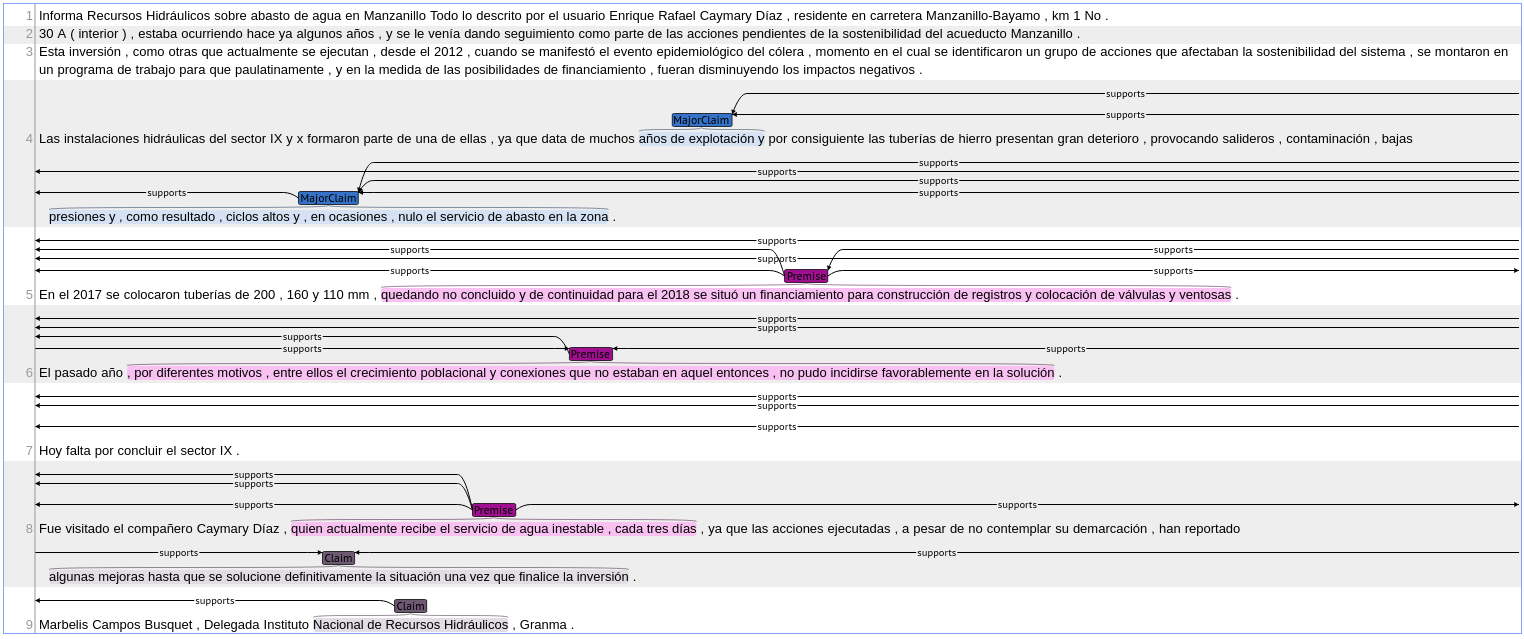
\includegraphics[scale=.4]{Graphics/persuasive_2019-01-25|informa-recursos-hidraulicos-sobre-abasto-de-agua-en-manzanillo|abasto-de-agua-en-manzanillo.png}
% 		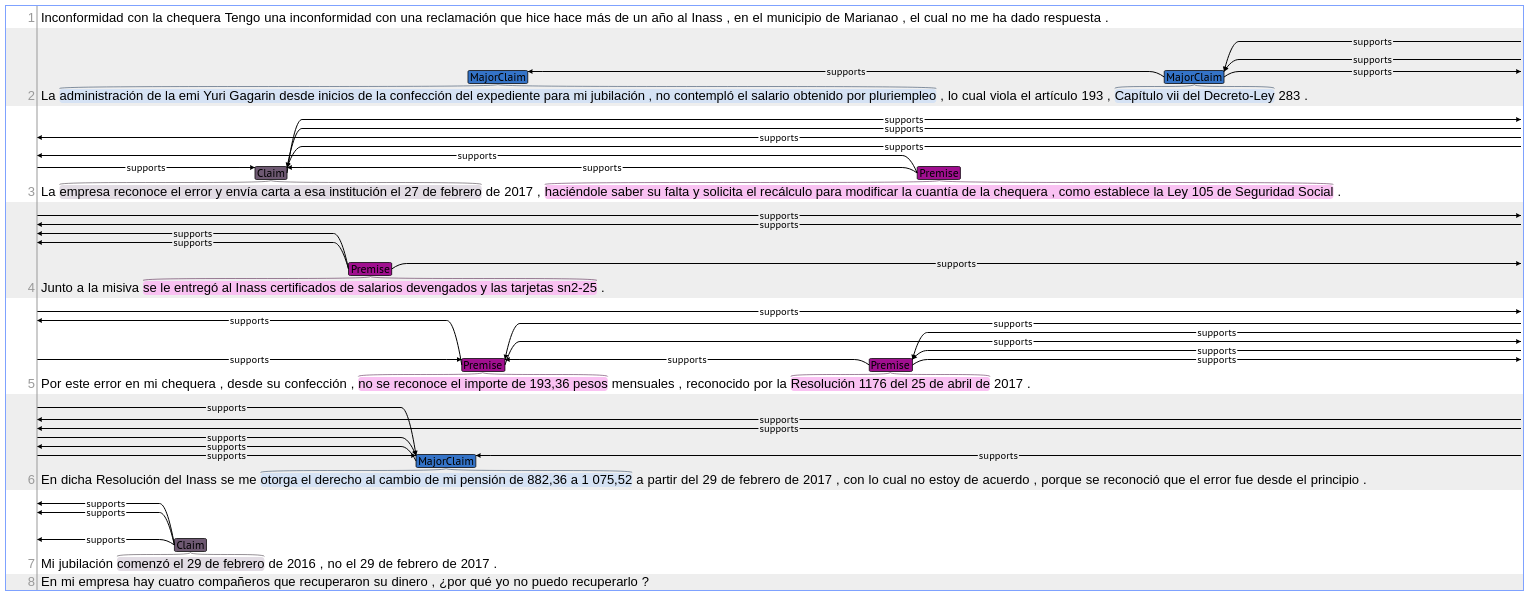
\includegraphics[scale=.4]{Graphics/persuasive_2019-03-22|inconformidad-con-la-chequera.png}
% 	    \caption{A}\label{fig:persuasive_granma_letters}
% 	\end{center}
% \end{figure}

Los ensayos argumentativos presentan una anotación de UDAs a un nivel de unidades de texto que pueden ser 
más pequeñas que oraciones y clasifican estas en las clases \emph{MajorClaim} (MC), \emph{Claim} (C) y \emph{Premise} 
(P). Las relaciones se clasifican en de \emph{supports} y \emph{attacks}. 

En general, se observa que se presentan problemas en la segmentación de UDAs debido al formato y dominio del texto.
Las cartas presentan una estrutura en donde al final se realiza una firma poniendo información acerca del remitente,
esta estructura no contribuye a la argumentación, pero el modelo en varias ocasiones detecta componentes en estas. 
Además de estos problemas de la estructura característica de la carta se encuentran otros. Entre los más 
encontrados se observa la extracción de supuestas UDAs que en su contenido no se encuentra un componente argumentativo, 
generalmente, estos elementos, si se expanden, pueden lograr establecer una mejor UDA.

Ejemplos malos:
\begin{itemize}
	\item \text{} [años de explotación y]$_{MC}$ 
	: Muy corto y no informativo. % 2019-01-25|informa-recursos-hidraulicos-sobre-abasto-de-agua-en-manzanillo|abasto-de-agua-en-manzanillo.txt.conll.link.conll.ann
	\item \text{} [en cada uno de los establecimientos de nuestra Cadena de Tiendas]$_{MC}$ 
	: Incompleto, mejora incorporando elementos de la izquierda (No a todos los productos con próxima fecha de vencimiento se le aplica rebaja de precios). % 2018-12-07|responde-trd-caribe-al-consumidor|a-proposito-de-la-proteccion-al-consumidor.txt.conll.link.conll.ann
	\item \text{} [Director División Grandes Centros]$_{MC}$ [TRD Caribe]$_{C}$ 
	: Mala clasificación y segmentación. %  2018-12-07|responde-trd-caribe-al-consumidor|a-proposito-de-la-proteccion-al-consumidor.txt.conll.link.conll.ann
	\item \text{} [Esperamos lo antes posible una solución]$_{P}$ 
	: En contexto, no contiene información que lo haga premisa % 2018-10-05|abasto-de-agua-en-manzanillo.txt.conll.link.conll.ann
	\item \text{} [no podemos permitir]$_{C}$ 
	: No establece una \emph{claim} % 2017-06-30|inass-reconoce-razon-de-ramiro-castellanos-por-inconformidad-con-trato-de-especialista-de-las-tunas|pregunta-quien-le-paga-su-jubilacion.txt.conll.link.conll.ann
\end{itemize}

Ejemplos buenos:
\begin{itemize}
	\item \text{} [no se le puede volver a despachar, tiene que ver a la administración (si está ahí en ese momento), 
	si no, regresar al día siguiente para que se le acredite lo sucedido]$_{MC}$ % 2021-02-26|inconvenientes-con-tarjetas-de-combustible-en-moneda-nacional.txt.conll.link.conll.ann
	\item \text{} [administración de la EMI Yuri Gagarin desde inicios de la confección del expediente para 
	mi jubilación, no contempló el salario obtenido por pluriempleo]$_{MC}$ % 2019-03-22|inconformidad-con-la-chequera.txt.conll.link.conll.ann
	\item pudiese [contribuir al ahorro de agua y la prestación de un mejor servicio]$_C$ % 2018-10-05|abasto-de-agua-en-manzanillo.txt.conll.link.conll.ann
	\item \text{} [es que estamos limitados de este servicio, y no desde hace un tiempo, es que nunca lo hemos tenido]$_P$ % 2018-05-18|sin-cobertura-en-guara-mayabeque.txt.conll.link.conll.ann
	\item \text{} [el número de carné de identidad que se encontraba en dicha base de datos correspondía a otra persona que
	fue reportada como fallecida]$_P$ % 2017-06-30|inass-reconoce-razon-de-ramiro-castellanos-por-inconformidad-con-trato-de-especialista-de-las-tunas|pregunta-quien-le-paga-su-jubilacion.txt.conll.link.conll.ann
\end{itemize}

Las relaciones anotadas por el modelo tienden a contener una gran cantidad de falsos positivos, además
dado que este conjunto de datos posee un gran desbalance en las etiquetas de las relaciones favoreciendo 
estas a las de \emph{supports}, el modelo no fue capaz de realizar anotaciones de \emph{attacks}, tanto en 
el conjunto de original de pruebas como en las cartas.

\subsection{Análisis de CDCP}

% \begin{figure}[h!]
% 	\begin{center}
% 		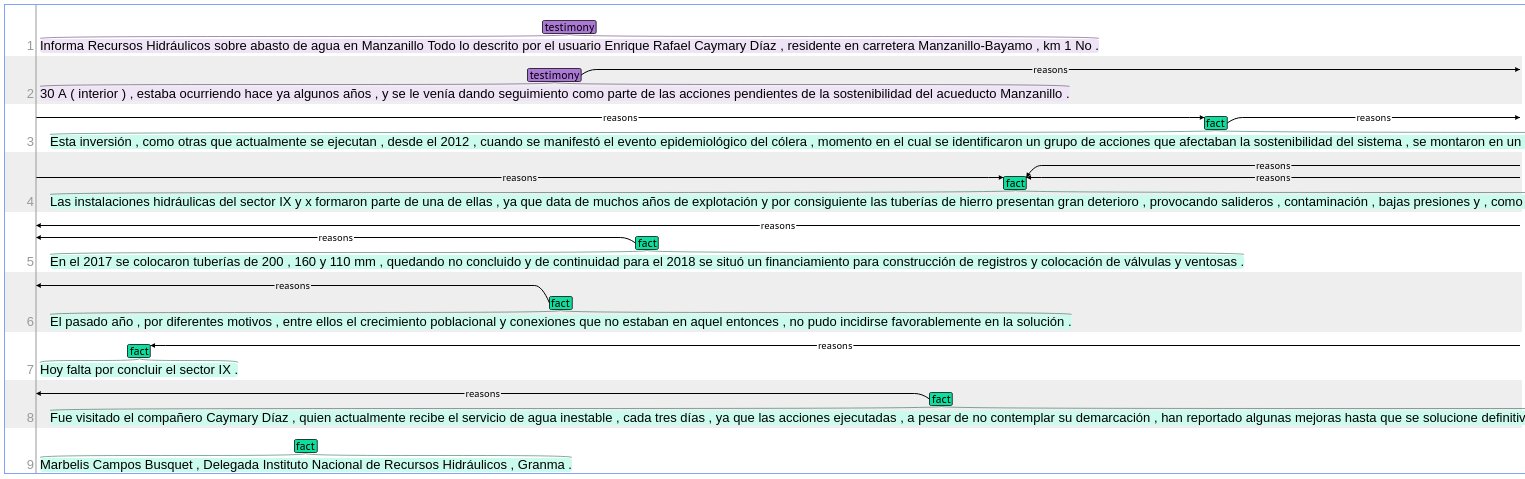
\includegraphics[scale=.4]{Graphics/cdcp_2019-01-25|informa-recursos-hidraulicos-sobre-abasto-de-agua-en-manzanillo|abasto-de-agua-en-manzanillo.png}
% 		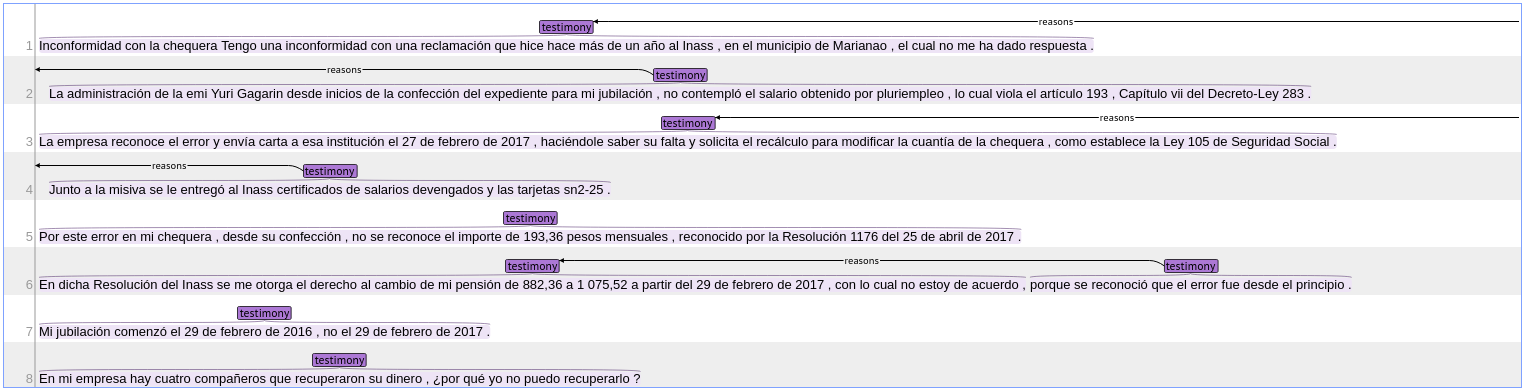
\includegraphics[scale=.4]{Graphics/cdcp_2019-03-22|inconformidad-con-la-chequera.png}
% 	    \caption{A}\label{fig:cdcp_granma_letters}
% 	\end{center}
% \end{figure}

CDCP realiza la segmentación de UDAs en la mayoría de las situaciones al separarlas por oraciones 
(solamente el 1\% de los tokens se encuentran fuera de una UDA),
estas son clasificadas en \emph{testimony} (T), \emph{fact} (F), \emph{policy} (P), \emph{reference} (R)
y \emph{value} (V). Las relaciones presentan dos tipos de relaciones \emph{evidences} y \emph{reasons}.

Los errores más comunes cometidos en la segmentación, dado el esquema utilizado, provienen del uso 
de signos de puntuación que no representan un cambio de oración, en estos casos se separa las UDA. También
existen errores de clasificación incorrecta, de, por ejemplo, \emph{testimony} que podrían ser \emph{fact}.

Ejemplos malos:
\begin{itemize}
	\item \text{} [\dots Bayamo, km 1 No.]$_T$ [30 A (interior), \dots]$_T$ 
	: Uso del \textbf{.} para abreviar número se toma como separador de UDA. % 2019-01-25|informa-recursos-hidraulicos-sobre-abasto-de-agua-en-manzanillo|abasto-de-agua-en-manzanillo.txt.conll.link.conll.ann
	\item \text{} [\dots ,desde el 1ro.]$_T$ [de marzo \dots]$_T$ 
	: Uso del \textbf{.} para abreviar primero se toma como separador de UDA. % 2019-05-24|le-retribuyen-la-diferencia-reclamada-de-su-pension|inconformidad-con-la-chequera.txt.conll.link.conll.ann
	\item \text{} [Junto a la misiva se le entregó al Inass certificados de salarios devengados y las tarjetas sn2-25.]$_T$ 
	: Se clasifica mejor como \emph{fact}. % 2019-03-22|inconformidad-con-la-chequera.txt.conll.link.conll.ann
	\item \text{} [Caridad Real Gutiérrez, Jefe de Trámites y Pensiones, Inass.]$_T$ 
	: Firma de la carta como elemento argumentaivo. % 2019-05-24|le-retribuyen-la-diferencia-reclamada-de-su-pension|inconformidad-con-la-chequera.txt.conll.link.conll.ann
\end{itemize}

Ejemplos buenos:
\begin{itemize}
	\item \text{} [En el 2017 se colocaron tuberías de 200, 160 y 110 mm, quedando no concluido y de 
	continuidad para el 2018 se situó un financiamiento para construcción de registros y colocación de 
	válvulas y ventosas.]$_F$ % 2019-01-25|informa-recursos-hidraulicos-sobre-abasto-de-agua-en-manzanillo|abasto-de-agua-en-manzanillo.txt.conll.link.conll.ann
	\item \text{} [Mi jubilación comenzó el 29 de febrero de 2016, no el 29 de febrero de 2017.]$_T$ % 2019-03-22|inconformidad-con-la-chequera.txt.conll.link.conll.ann
	\item \text{} [No se sabe cuánto queda, lo que obliga al cliente a estar haciendo cuentas constantemente.]$_F$ % 2021-05-07|servicentros-operan-diversos-medios-de-pago-electronicos|inconvenientes-con-tarjetas-de-combustible-en-moneda-nacional.txt.conll.link.conll.ann
\end{itemize}

Las relaciones presentes disminuyen en cantidad en comparación con lo visto en los textos anotados con el modelo 
entrenado con Ensayos Argumentativos. Prevaleciendo las relaciones de \emph{reasons}. A consideración del autor,
la cantidad de los falsos positivos son menores que el modelo de Ensayos Argumentativos.

\subsection{Análisis AbsTRCT}

% \begin{figure}[h!]
% 	\begin{center}
% 		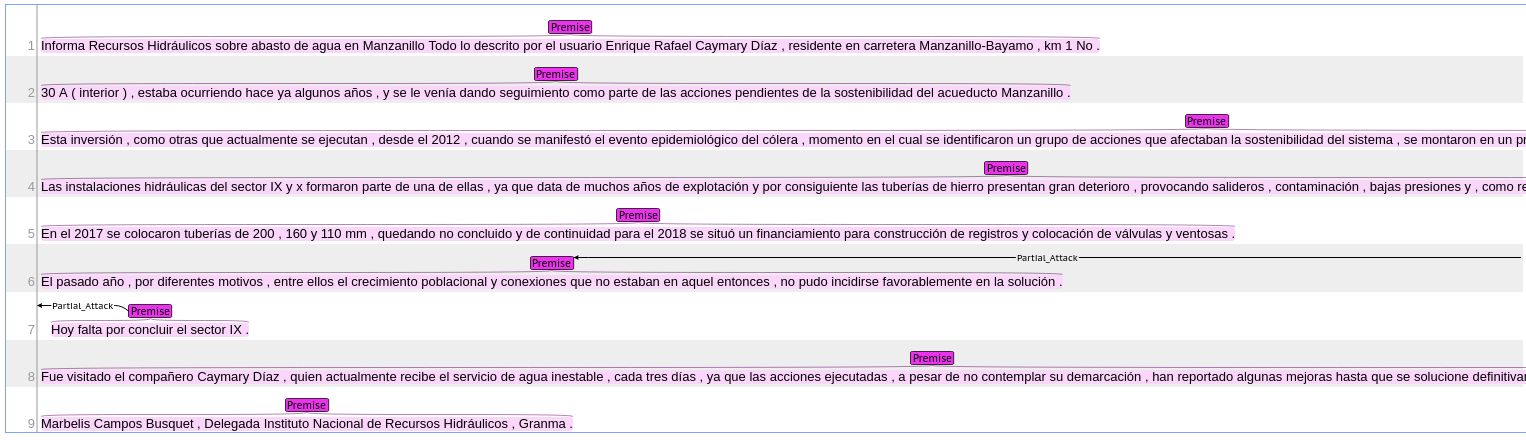
\includegraphics[scale=.4]{Graphics/abstrct_2019-01-25|informa-recursos-hidraulicos-sobre-abasto-de-agua-en-manzanillo|abasto-de-agua-en-manzanillo.png}
% 		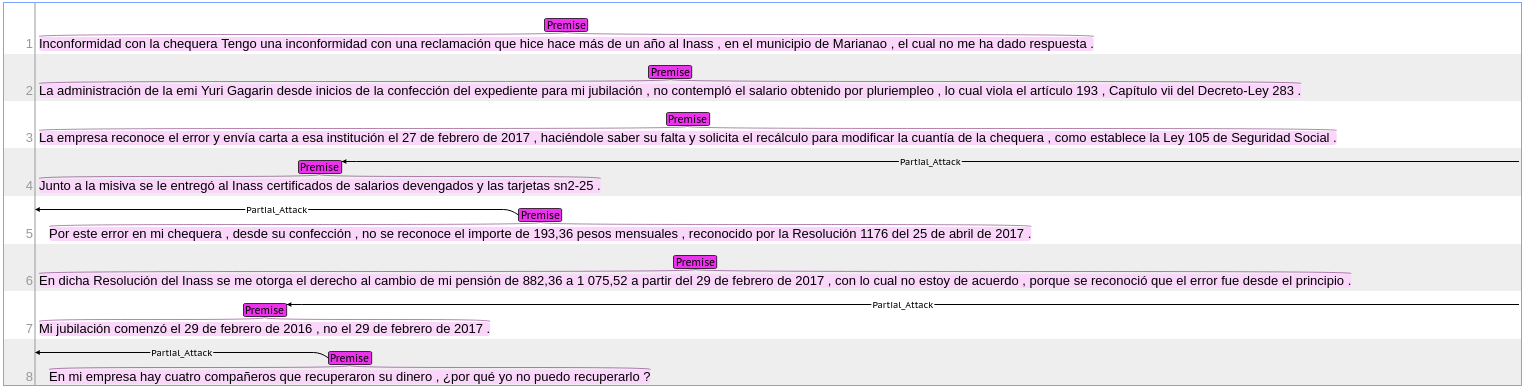
\includegraphics[scale=.4]{Graphics/abstrct_2019-03-22|inconformidad-con-la-chequera.png}
% 		\caption{A}\label{fig:abstrct_granma_letters}
% 	\end{center}
% \end{figure}

El conjunto de datos presenta un estilo de segmentación de UDAs en donde se anotan 
secciones de textos más grandes que en Ensayos Argumentativos, aunque no necesariamente 
todas las oraciones o la oración completa es considerada argumentativa. 
Estas se clasifican igual que Ensayos Argumentativos, aunque 
en este conjunto de datos se presenta un desbalance de etiquetas grande, favoreciendo 
a las \emph{Premise} y las \emph{Claim}, dejando sin representación casi a \emph{MajorClaim}
(menor del 1\% de las etiquetas BIOES), lo que trajo como consecuencia que el modelo no fuera 
capaz de diferenciar este tipo de UDA. Las relaciones se presentaron como \emph{partial-attack},
\emph{attack} y \emph{support}, influenciadas también por la poca cantidad de relaciones de \emph{attack}.

En la clasificación de UDAs se evidencia una gran cantidad de \emph{Premise}.

Ejemplos malos:
\begin{itemize}
	\item \text{} [\dots Calle 14, apto.]$_P$ [4 entre Zapata y 23, \dots]$_T$ 
	: Uso del \textbf{.} para abreviar apartamento se toma como separador de UDA. % 2017-07-07|parque-en-pleno-deterioro-en-plaza.txt.conll.link.conll.ann
	\item \text{} [, Director División Grandes Centros TRD Caribe.]$_C$ 
	: Mala clasificación con mala segmentación y detección de \emph{claim} en firma de carta. 
\end{itemize}

Ejemplos buenos:
\begin{itemize}
	\item \text{} [Esta situación pudo haberse evitado y no podemos permitir que hechos como este ocurran pues, 
	empañan la imagen de la institución que está destinada a brindar un servicio con calidad a la población en 
	general y en especial a los jubilados y pensionados.]$_P$ % 2017-06-30|inass-reconoce-razon-de-ramiro-castellanos-por-inconformidad-con-trato-de-especialista-de-las-tunas|pregunta-quien-le-paga-su-jubilacion.txt.conll.link.conll.ann
	\item \text{} [Esta respuesta considera sin razón la preocupación de un lector, 
	¿así debe terminar la inquietud de un ciudadano, que confía en las instituciones con que cuenta la 
	sociedad para enfrentar sus problemas?]$_C$ % 2017-05-12|cimex-se-dirige-a-limitado-fisico-motor|llamado-a-evaluar-situacion-de-piezas-y-baterias-para-equipos-motorizados-de-discapacitados.txt.conll.link.conll.ann
\end{itemize}

Las relaciones tienen la menor cantidad de elementos de los otros conjuntos de datos, proliferando
las relaciones de \emph{support}. En las clasificadas como \emph{partial-attack} se evidenció, a 
consideración del autor, una baja precisión. Por ejemplo 
[\emph{cierto que la responsabilidad es de todos, pero la institucional es de la Dirección de Comunales.}]
ataca a [\emph{Antonio Blanco, Director de Servicios Comunales Plaza,}].

\subsection{Resultados}

Se considera que el conjunto de datos CDCP se ajusta mejor a las características de las Cartas 
a la Dirección. Este presenta orígenes similares, es contenido generado por usuarios en una plataforma
web, y, por lo tanto, presenta un conjunto de etiquetas de UDAs que se ajustan más a lo observado 
en las cartas. También las cartas presentan un alto contenido argumentativo, por lo que marcar 
todas las oraciones como argumentativas no constituye una fuente grande de errores, aunque esta 
parte puede ser mejorada. Una desventaja de este esquema sobre otros es la carencia de una 
clasificación de las relaciones que implique un ataque, aunque esto se cubre con el hecho de 
que en los conjuntos en donde existen estas los resultados son bastante pobres en ese aspecto. La cantidad 
y calidad de relaciones, aunque tiene bastante espacio para mejorar, es aceptable dada la dificultad 
del problema en EA.

Con CDCP se obtiene una visión general de la argumentación, aunque si se desea obtener algo 
más específico podría considerarse el modelo de Ensayos Argumentativos. La ventaja de este 
modelo en la extracción y clasificación de UDA es que utiliza un conjunto de etiquetas que 
podría considerarse universal en la argumentación y además reduce el espacio de búsqueda de 
oraciones a segmentos de palabras, aunque estos puedan estar sujetos a errores. 

La versión de AbsTRCT constituye el modelo con menor rendimiento. La clasificación
de UDAs presenta una gran desproporción hacia \emph{Premise} dejando muchas \emph{Claim}
sin ser conrrectamente clasificadas. Sobre las relaciones muestra un nivel muy bajo de 
relaciones por documento, en relación a las que se podrían formar.


\backmatter

\begin{conclusions}

% Como se cumplieron los objetivos de la introduccion
% Lo que hice para que puede servir, 
% en que escenarios, 
% es competitivo con el estado del arte, 
% por qué sí o por qué no
    
En el trabajo se logró la extracción de estructuras argumentativas en los textos de las 
Cartas a la Dirección del periódico Granma. Para esto se 
extrajeron los textos de las Cartas creando un conjunto de datos
conteniendo, no solo el texto de las cartas, si no, los comentarios 
escritos por los usuarios e información sobre la carta a la que responde, si es una respuesta.
Se creó un software que puede ser utilizado no solo para el trabajo con las Cartas a la Dirección, si no
que este permite un uso general para las tareas de proyección de corpus y trabajo relacionados a la EA.
Este permite incorporar nuevas componentes haciendo posible una extensión simple y desacoplada. 
Para la anotación de las estructuras se crearon conjuntos de datos en español a partir de conjuntos 
anotados en inglés para poder 
tener datos con los cuales entrenar los modelos propuestos. Estos modelos, uno encargado 
de la segmentación y clasificación de las UDAs, y otro de la extracción y clasificación de las 
relaciones entre estas, fueron utilizados para la anotación de los textos extraídos.
Los resultados obtenidos en la tarea de segmentación se encuentran al nivel del estado del arte,
en las demás tareas no se encontraron comparaciones directas al enfoque tomado en la propuesta,
aunque no teniendo en cuenta esto, se obtienen comparativas inferiores en la clasificación
de UDAs y en la clasificación de relaciones, aunque se supera la métrica de predicción de enlace. 
Los resultados obtenidos del procesamiento de las Cartas a la Dirección son considerados 
aceptables por autor. 

\end{conclusions}

\begin{recomendations}
    Recomendaciones

    \begin{enumerate}
        \item Usar metodos de Graph Neural Networks para modelar las relaciones entre las UDA. (Actualmente las relaciones extra'idas son independientes)
        \item Ajustar (Tune) awesome-align con ingl'es-español.
        \item Usar otros embeddings para la representación de palabras (BERT, SciBERT, RoBERTa).
        \item Desplegar un servidor Brat para socializar los resultados y permitir que los investigadores perfeccionen las anotaciones.
        \item Validación externa con lingüistas que permitan generalizar el uso del modelo.
    \end{enumerate}
\end{recomendations}

% biber
\printbibliography[heading=bibintoc]

% natlib
% \bibliographystyle{myplainnat}
% \bibliography{Bibliography}

\end{document}